%definira klasu dokumenta 
\documentclass[12pt]{report} 

%prostor izmedu naredbi \documentclass i \begin{document} se zove uvod. U njemu se nalaze naredbe koje se odnose na cijeli dokument

%osnovni LaTex ne može riješiti sve probleme, pa se koriste različiti paketi koji olakšavaju izradu željenog dokumenta
\usepackage[croatian]{babel} 
\usepackage{amssymb}
\usepackage{amsmath}
\usepackage{txfonts}
\usepackage{mathdots}
\usepackage{titlesec}
\usepackage{array}
\usepackage{lastpage}
\usepackage{etoolbox}
\usepackage{longtable, tabu}
\usepackage{color, colortbl}
\usepackage{adjustbox}
\usepackage{geometry}
\usepackage[classicReIm]{kpfonts}
\usepackage{hyperref}
\usepackage{fancyhdr}
\usepackage{graphicx}
\usepackage{wrapfig,lipsum}
\usepackage{subcaption}
\usepackage{float}
\usepackage{setspace}
\restylefloat{table}


\patchcmd{\chapter}{\thispagestyle{plain}}{\thispagestyle{fancy}}{}{} %redefiniranje stila stranice u paketu fancyhdr

%oblik naslova poglavlja
\titleformat{\chapter}{\normalfont\huge\bfseries}{\thechapter.}{20pt}{\Huge}
\titlespacing{\chapter}{0pt}{0pt}{40pt}


\linespread{1.3} %razmak između redaka

\geometry{a4paper, left=1in, top=1in,}  %oblik stranice

\hypersetup{ colorlinks, citecolor=black, filecolor=black, linkcolor=black,	urlcolor=black }   %izgled poveznice


%prored smanjen između redaka u nabrajanjima i popisima
\newenvironment{packed_enum}{
	\begin{enumerate}
		\setlength{\itemsep}{0pt}
		\setlength{\parskip}{0pt}
		\setlength{\parsep}{0pt}
	}{\end{enumerate}}

\newenvironment{packed_item}{
	\begin{itemize}
		\setlength{\itemsep}{0pt}
		\setlength{\parskip}{0pt}
		\setlength{\parsep}{0pt}
	}{\end{itemize}}


%boja za privatni i udaljeni kljuc u tablicama
\definecolor{LightBlue}{rgb}{0.9,0.9,1}
\definecolor{LightGreen}{rgb}{0.9,1,0.9}


%podesavanje zaglavlja i podnožja

\pagestyle{fancy}
\lhead{Programsko inženjerstvo}
\rhead{HGSStracks}
\lfoot{Havana}
\cfoot{stranica \thepage/\pageref{LastPage}}
\rfoot{\today}
\renewcommand{\headrulewidth}{0.2pt}
\renewcommand{\footrulewidth}{0.2pt}


\begin{document} 
	
	
	
	\begin{titlepage}
		\begin{center}
			\vspace*{\stretch{1.0}} %u kombinaciji s ostalim \vspace naredbama definira razmak između redaka teksta
			\LARGE Programsko inženjerstvo\\
			\large Ak. god. 2020./2021.\\
			
			\vspace*{\stretch{3.0}}
			
			\huge HGSStracks\\
			\Large Dokumentacija, Rev. \textit{1}\\
			
			\vspace*{\stretch{12.0}}
			\normalsize
			Grupa: \textit{Havana}\\
			Voditelj: \textit{Mia Stojak}\\
			
			
			\vspace*{\stretch{1.0}}
			Datum predaje: \textit{13.11.2020.}\\
	
			\vspace*{\stretch{4.0}}
			
			Nastavnik: \textit{Hrvoje Nuić}\\
		
		\end{center}

	
	\end{titlepage}

	
	\tableofcontents

	\chapter{Dnevnik promjena dokumentacije}
		
		\textbf{\textit{Kontinuirano osvježavanje}}\\
				
		
		\begin{longtabu} to \textwidth {|X[2, l]|X[13, l]|X[3, l]|X[3, l]|}
			\hline \multicolumn{1}{|l|}{\textbf{Rev.}}	& \multicolumn{1}{l|}{\textbf{Opis promjene/dodatka}} & \multicolumn{1}{|l|}{\textbf{Autori}} & \multicolumn{1}{l|}{\textbf{Datum}} \\[3pt] \hline
			\endfirsthead
			
			\hline \multicolumn{1}{|l|}{\textbf{Rev.}}	& \multicolumn{1}{l|}{\textbf{Opis promjene/dodatka}} & \multicolumn{1}{|l|}{\textbf{Autori}} & \multicolumn{1}{l|}{\textbf{Datum}} \\[3pt] \hline
			\endhead
			
			\hline 
			\endlastfoot
			
			0.1 & Napravljen predložak.	& Stojak & 09.10.2020. 		\\[3pt] \hline 
			0.2.1	& Napisan dio Opis projektnog zadatka. & Stojak & 14.10.2020. 	\\[3pt] \hline 
			0.2.2	& Proširen Opis projektnog zadatka. & Kovačić & 6.11.2020. 	\\[3pt] \hline
			0.3.1 & Funkcionalni zahtjevi korisnika\newline 15 Obrazaca uporabe & Boras & 21.10.2020. \\[3pt] \hline
			0.3.2 & Funkcionalni zahtjevi voditelja spasioca\newline 3 Obrazaca uporabe & Škrabić & 21.10.2020. \\[3pt] \hline
			0.3.3 & Funkcionalni zahtjevi
			neregistriranog korisnika\newline 3 Obrazaca uporabe & Mlakić & 21.10.2020. \\[3pt] \hline 
			0.3.4 & Funkcionalni zahtjevi baze podataka\newline 3 Obrazaca uporabe  & Gusar & 22.10.2020. \\[3pt] \hline
			0.3.5 & Funkcionalni zahtjevi dispečera\newline 3 Obrazaca uporabe & Kovačić & 23.10.2020. \\[3pt] \hline
			0.3.6 & Funkcionalni zahtjevi administratora\newline 3 Obrazaca uporabe & Stojak & 24.10.2020. \\[3pt] \hline
			0.3.7 & Funkcionalni zahtjevi spasioca\newline 3 Obrazaca uporabe & Kovač & 24.10.2020. \\[3pt] \hline
			0.3.8 & Ostali zahtjevi & Boras & 07.11.2020. \\[3pt] \hline
			0.4 & Dijagrami obrazaca uporabe & Mlakić & 08.11.2020. \\[3pt] \hline 
			0.5 & Sekvencijski dijagrami & Škrabić & 08.11.2020. \\[3pt] \hline 
			0.6 & Arhitektura i dizajn sustava\newline Baza podataka,opis tablica\newline Dijagram baze podataka & Gusar & 07.11.2020. \\[3pt] \hline
			0.8 & Dijagram i opis razreda & Kovačić & 13.11.2020. \\[3pt] \hline
			\textbf{1.0} & Verzija samo s bitnim dijelovima za 1. ciklus & Stojak & 12.11.2020. 
			\\[3pt] \hline
			\textbf{1.1} & Dijagram stanja & Kovačić & 11.1.2021. 
			\\[3pt] \hline
			\textbf{1.2} & Dijagram aktivnosti & Kovačić & 11.1.2021.
			\\[3pt] \hline
			\textbf{1.3} & Dijagram razmještaja & Kovačić & 12.1.2021.
			\\[3pt] \hline
			\textbf{1.4} & Dijagram komponenti & Kovačić & 12.1.2021.
			\\[3pt] \hline
			\textbf{1.8} & Upute za puštanje u pogon & Kovačić & 12.1.2021.
			\\[3pt] \hline
			\textbf{1.9} & Zaključak & Kovačić & 12.1.2021.
			\\[3pt] \hline
			\textbf{2} & Verzija samo s bitnim dijelovima za 2. ciklus & Stojak & 14.1.2021.
			
		\end{longtabu}
	
	
		
	\chapter{Opis projektnog zadatka}
		{Cilj ovog projekta je napraviti web aplikaciju HGSStracks koja olakšava koordinaciju rada svih ljudi, spasioca ili dispečera, aktivnih na akciji spašavanja. Aplikacija korisniku omogućava praćenje akcije spašavanja osobe prijavljene kao nestale. Također omogućuje nadležnoj osobi koordinaciju spasioca na terenu u stvarnom vremenu. Aplikacija služi kao potpuna postojeće aplikacije napravljene od strane organizacije "Hrvatski Crveni križ"(nadalje u tekstu HCK), koja pruža razne informacije vezane uz spašavanje ljudi, koje je zadesila nesreća, te kako medicinski pomoći osobi ako je potrebno.\\
			\begin{figure}[h!]
				\centering
				\begin{subfigure}[b]{0.3\linewidth}
					\centering
					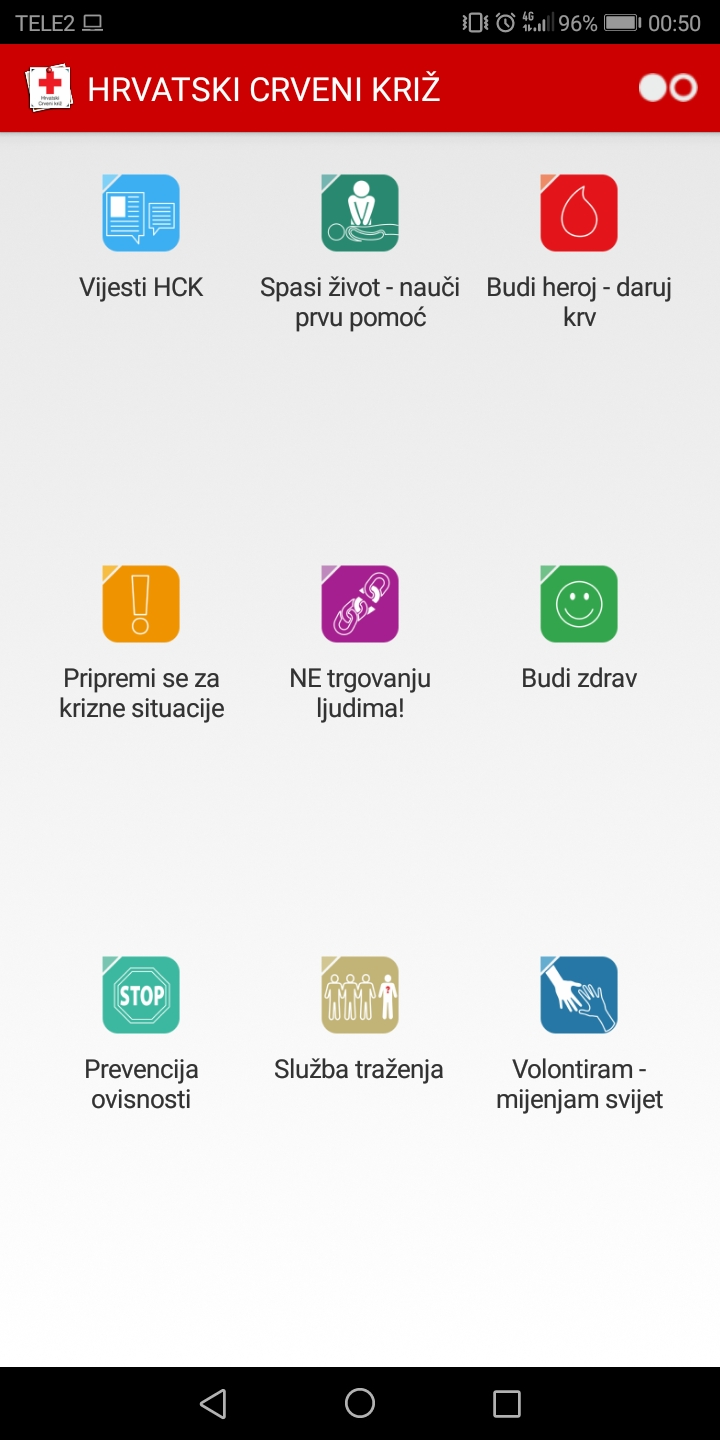
\includegraphics[scale=0.1]{./slike/crv1.jpg}
					\caption{\tiny Početna stranica aplikacije HCK}
					\label{fig:sub-first}
				\end{subfigure}
				\begin{subfigure}[b]{0.3\linewidth}
					\centering
					
\includegraphics[scale=0.1]{./slike/crv2.jpg}
					\caption{\tiny Podstranica aplikacije HCK s uputama za prvu pomoć}
					\label{fig:sub-second}
				\end{subfigure}
				\begin{subfigure}[b]{0.3\linewidth}
					\centering
					
\includegraphics[scale=0.1]{./slike/crv3.jpg}
					\caption{\tiny Podstranica aplikacije HCK s knjigom nestalih te opisom rada službe za spašavanje}
					\label{fig:sub-third}
				\end{subfigure}
			\caption{Prikaz postojeće aplikacije HCK}
			\label{fig:fig}
			\end{figure}\\
			
			Cilj aplikacije je brzo i jednostavno reagiranje na prijavu nesreće ili nestanka osobe, te umanjenje potrebnog vremena za spašavanje žrtava nesreće. Također odvajamo uloge, i zadatke po ulogama, kako bi osobe na terenu znale što su dužne odraditi, gdje trebaju doći i tko je u opasnosti.\\
		Prilikom pokretanja sustava korisnike se pita za autentifikaciju kredencija ako imaju već izrađen i autoriziran račun od strane administratora.\\
		Neregistrirani korisnici mogu se registrirati s postojećim računom ili kreirati novi račun pritiskom na gumb – Registracija. 
		\\\\Za registraciju korisnik bira ulogu koju želi obnašati (spasilac, dispečer) te su potrebni sljedeći podaci:}


		\begin{packed_item}
			\item {korisničko ime} 
			\item {fotografija}
			\item {lozinka}
			\item {ime}
			\item {prezime}
			\item {broj mobitela}
			\item {email adresa}
		\end{packed_item}
	
		{Prilikom registracije korisnika zahtjev se šalje administratoru koji ju je dužan odobriti ili odbiti. Ovisno o ulozi koju je izabrao, te mu je ona odobrena od administratora, registracijom u sustav korisniku se dodjeljuju određena prava ovisno o njegovoj ulozi u aplikaciji.\\
			
			Postoje 4 vrste korisnika popisana silazno prema razini ovlasti koje imaju za vrijeme korištenja aplikacije: Administrator, Dispečer, Voditelj, Spasilac.\\ 
			
			\begin{wrapfigure}{l}{0.25\textwidth}
				\centering
				
\includegraphics[width=0.25\textwidth]{./slike/spasioc.png}
				\caption{Ikona spasioca}
			\end{wrapfigure}
			\textbf{Spasilac} pripada nekoj stanici i redovito je dužan osvježavati podatak o dostupnosti za akcije spašavanja koje je moguće da sam podesi na svojem profilu ili ako je stavljen u akciju spašavanja od strane dispečera automatski je postavljeno u "Nedostupan". Spasilac se sam može odazvati na akciju ako zadovoljava tražene kriterije koje je postavio Dispečer; može potvrditi zahtjev poslan od dispečera ako on smatra da je potreban akciji a on se nije javio na istu.\\ Tijekom akcije na karti ostavlja trag kojim prolazi (trag ostavlja pomoću GPS-a na mobilnom telefonu) i time pokazuje svoj položaj Dispečeru u obliku toplinske karte. Na karti mu se prikazuju zadaci koje treba obaviti zadane od strane Voditelja ili Dispečera, privremene i stalne postaje te trenutna pozicija ostalih spasilaca aktivnih na akciji spašavanja. Spasilac u njegovoj aktivnoj akciji ima mogućnost ostavljanja komentara na ruti kroz koju prolazi za ostale sudionike spašavanja.\\
			
			
			\begin{wrapfigure}{r}{0.25\textwidth}
				\centering
				
\includegraphics[width=0.25\textwidth]{./slike/leader.png}
				\caption{Ikona voditelja spasioca}
			\end{wrapfigure}
			\textbf{Voditelj} spasioca je glavni spasilac u stanici. On je i sam spasilac, no ima specifične ovlasti koje "običan" spasilac nema. Pod posebne ovlasti Voditelja spada definiranje načina na koji su određeni Spasioci vlastite stanice voditelja osposobljeni obavljati akcije spašavanja unesrećene osobe. Ovisno o načinu izvođenja spašavanja spasilac ima definiranu veličinu i intenzitet područja kojeg može u trenu vidjeti na karti u aplikaciji.\\
			Vrste izvođenja spašavanja su:
			
			\begin{packed_item}
				\item {Auto} 
				\item {Bicikl}
				\item {Pješice}
				\item {Pas}
				\item {Dron}
				\item {Helikopter}
				\item {Plovilo}
			\end{packed_item}
		
		
			\begin{wrapfigure}{l}{0.25\textwidth}
				\centering
				
\includegraphics[width=0.25\textwidth]{./slike/Dispatch.png}
				\caption{Ikona dispečera}
			\end{wrapfigure}
			\textbf{Dispečer} je osoba odgovorna za raspoređivanje osoblja i nadziranja rada cijelog sustava akcija spašavanja osoba iz jednog centriranog odjela udaljenog od samih akcija.Slijedno dostavi prijave nesreće,dužan je otvoriti akciju spašavanja s informacijama o nestaloj osobi, te nakon što je osoba pronađena i pružena joj je potrebna pomoć završava akciju te je sprema u bazu "riješenih" akcija. Početkom akcije ima uvid u broj dostupnih spasilaca po stanicama u blizini nestanka osobe te ima mogućnost poslati zahtjev za uključivanje spasilaca u akciju,i ako procjenom zaključi da je potreban veći broj spasioca može dodati spasioce iz udaljenih stanica, te ih može ukloniti s akcije u slučaju njihovih upitnih postupaka za vrijeme spašavanja. Prilikom slanja zahtijeva, dispečer definira način sudjelovanja spasilaca (ako postoji mogućnost u stanici gdje je spasilac stacioniran), zadaje im individualne zadatke te ima mogućnost postavljanja dodatnih komentara za zadate ; izbjegavanje određenih stvari, moguće alergije na penicilin itd. \\ Mogući zadatci su:
			
			\begin{packed_item}
				\item {Prođi određenom rutom} 
				\item {Postavi privremenu postaju}
				\item {Osvježi zalihe u privremenoj postaji}
				\item {I sl.}
			\end{packed_item}
			
			Uz zadatke zadane spasiocima na karti prikazuju mu se i tragovi svih aktivnih spasioca unutar zadnja 2 sata. Dispečer ima mogućnost uključivanja prikaza toplinske karte temeljene na dosadašnjim prijeđenim tragovima spasioca i načinima na koje sudjeluju(navedenim u paragrafu Voditelja spasioca).\\
		
			\textbf{Administrator} može vidjeti popis svih registriranih korisnika sustava te njihove osobne podatke, izmjenjivati dodijeljena prava i određene podatke. U slučaju zatražene registracije vrši provjeru kredencija mogućeg novog korisnika te je potvrđuje, i dodjeljuje potrebne ovlasti ako su one odobrene od strane samog HGSS-a; Voditelj, Dispečer, Spasilac. \\ Jedan od zadataka administratora je pregled podataka i njihove točnosti u samom sustavu te izrada sigurnosne kopije na udaljenom mjestu za slučaj pada samog sustava. U slučaju trajnog zatvaranja tj. otvaranja stanice na karti dužan je podatke korigirati u sustavu tj. bazi. U slučaju pada sustava administrator pregledava razlog istog, te nakon otklanjanja problema ponovno pokreće sustav i ažurira podatke ovisno o promjenama do kojih je došlo između pada i ponovnog pokretanja sustava.\\}\\*
		
		
	\chapter{Specifikacija programske potpore}
		
	\section{Funkcionalni zahtjevi}
			
			\noindent \textbf{Dionici:}
			
			\begin{packed_enum}
				
				\item Vlasnik(naručitelj)
				\item Administrator	
				\item Korisnici aplikacije
				\begin{packed_enum}
					\item Dispečer
					\item Voditelj spasioca
					\item Spasilac
				\end{packed_enum}
				\item Razvojni tim
				
			\end{packed_enum}
			
			\noindent \textbf{Aktori i njihovi funkcionalni zahtjevi:}
			
			
			\begin{packed_enum}
				
				\item  \underbar{Neregistrirani/neprijavljeni korisnik može:}
				
				\begin{packed_enum}
					\item otvoriti stranicu za registraciju i registrirati se ako već nije
					\item otvoriti stranicu za prijavu i prijaviti se ako je već registriran
				\end{packed_enum}
			
				\item  \underbar{Korisnik aplikacije (inicijator) može:}
		
				\begin{packed_enum}
				
					\item Prijaviti se u sustav
					\item Vidjeti i mijenjati osobne podatke
					\item Izbrisati korisnički račun
				
				\end{packed_enum}
				
				\item  \underbar{Administrator (inicijator) može:}
				
				\begin{packed_enum}
					\item potvrđivati zahtjeve za registraciju
					\item vidjeti popis svih registriranih korisnika i njihovih osobnih podataka.
					\item mijenjati dodijeljena prava korisnicima
					\item mijenjati i uređivati osobne podatke korisnika
					\item Dodjeljivati status voditelja postaje spasiocu
					\item uređivati i dodavati informacije vezane uz stanice
				\end{packed_enum}
				
				\item  \underbar{Dispečer(inicijator) može:}
				
				\begin{packed_enum}
					
					\item Otvoriti akciju spašavanja, te dodati informacije o nestaloj osobi
					\item Slati zahtjev za uključivanje određenog spasioca u akciju spašavanja
					\item Dodavati/mijenjati zadatke pojedinih spasilaca u trenutnoj akciji
					\item Slati pomoćne komentare uz nove zadatke spasioca
					\item Ukloniti određenog spasioca s trenutne akcije spašavanja
					\item Označiti kraj akcije spašavanja (kada je osoba nađena)
					
				\end{packed_enum}
			
				\item \underbar{Spasioc(inicijator) može:}
			
				\begin{packed_enum}
					\item Sudjelovati u akciji spašavanja
					\item Osvježavati podatak o dostupnosti za akcije
					\item Pregledavati njemu zadane zadatke
					\item Postaviti privremenu postaju na karti
					\item Ostaviti komentare na akciji spašavanja na karti za ostale sudionike
				\end{packed_enum}
			
				\item \underbar{Voditelj spasioca(inicijator) može:}
			
				\begin{packed_enum}
					\item Definirati spasiocima u svojoj stanici na koji su način osposobljeni voditi spašavanje(auto, bicikl, pješke, pas, dron, helikopter, brod)
					\item Sudjelovati u akciji spašavanja
				\end{packed_enum}
			
				\item \underbar{Baza podataka(sudionik):}
			
				\begin{packed_enum}
					\item Sprema podatke o korisnicima aplikacije te sprema njihove ovlasti
					\item Sprema podatke o postojećim stanicama
					\item Sprema podatke o već provedenim akcijama te onima koje su još u tijeku
					\item Sprema podatke o lokacijama spasilaca
				\end{packed_enum}
			\end{packed_enum}
			
			\eject 
			
			
				
			\subsection{Obrasci uporabe\\}

				
				\noindent \underbar{\textbf{UC1 - Slanje zahtjeva za registraciju}}
				\begin{packed_item}
					
					\item \textbf{Glavni sudionik: }Korisnik
					\item  \textbf{Cilj:} Poslati zahtjev za registraciju
					\item  \textbf{Sudionici:} Baza podataka
					\item  \textbf{Preduvjet:} -
					\item  \textbf{Opis osnovnog tijeka:}
					
					\item[] \begin{packed_enum}
						
						\item Korisnik otvara opciju za registraciju.
						\item Korisnik unosi potrebne podatke za registraciju.
						\item Korisnik šalje zahtjev za registraciju
						\item Baza podataka se ažurira
						\item Sustav obavještava korisnika da je zahtjev poslan
						
					\end{packed_enum}
					
					\item  \textbf{Opis mogućih odstupanja:}
					
					\item[] \begin{packed_item}
						
						\item[2.a] Odabir postojećeg korisničkog imena ili e-maila
						\item[] \begin{packed_enum}
							
							\item Obavještavamo korisnika da je korisničko ime ili e-mail nedostupan te ga vraćamo na stranicu za registraciju.
						\end{packed_enum}
							
						\item[2.b] Unos neispravnog e-mail računa
						\item[] \begin{packed_enum}
							
							\item Obavještavamo korisnika da je uneseni e-mail neispravan te ga vraćamo na stranicu za registraciju.\\						
						\end{packed_enum}
					\end{packed_item}
				\end{packed_item}
			
				\noindent \underbar{\textbf{UC2 - Prikaz zahtjeva za registraciju}}
				\begin{packed_item}
					
					\item \textbf{Glavni sudionik: }Administrator
					\item  \textbf{Cilj:} Pregledati sve zahtjeve za registraciju
					\item  \textbf{Sudionici:} Baza podataka
					\item  \textbf{Preduvjet:} -
					\item  \textbf{Opis osnovnog tijeka:}
					
					\item[] \begin{packed_enum}
						
						\item Administrator odabire opciju "Prikaži zahtjeve za registraciju"
						\item Prikazuju se svi poslani zahtjevi za registraciju
					\end{packed_enum}
				\end{packed_item}
			\newpage
				\noindent \underbar{\textbf{UC3 - Reguliranje zahtjeva za registraciju}}
				\begin{packed_item}
					
					\item \textbf{Glavni sudionik: }Administrator
					\item  \textbf{Cilj:} Regulirati zahtjeve za registraciju
					\item  \textbf{Sudionici:} Baza podataka
					\item  \textbf{Preduvjet:} Administrator pregledava zahtjeve za registraciju
					\item  \textbf{Opis osnovnog tijeka:}
					
					\item[] \begin{packed_enum}
						
						\item Administrator odabire prikaz zahtjeva za registraciju
						\item Administrator prihvaća/odbija zahtjev za registraciju
						\item Baza podataka se ažurira\\
					\end{packed_enum}
				\end{packed_item}
				\noindent \underbar{\textbf{UC4 - Prijava u sustav}}
				\begin{packed_item}
					
					\item \textbf{Glavni sudionik: }Korisnik
					\item  \textbf{Cilj:} Dobiti pristup korisničkom sučelju
					\item  \textbf{Sudionici:} Baza podataka
					\item  \textbf{Preduvjet:} Registracija
					\item  \textbf{Opis osnovnog tijeka:}
					
					\item[] \begin{packed_enum}
						
						\item Unos korisničkog imena i lozinke
						\item Potvrda o ispravnosti unesenih podataka
						\item Pristup korisničkim funkcijama
					\end{packed_enum}
					
					\item  \textbf{Opis mogućih odstupanja:}
					
					\item[] \begin{packed_item}
						
						\item[2.a] Uneseni podaci su neispravni
						\item[] \begin{packed_enum}
							
							\item Sustav obavještava korisnika o neispravno unesenim podacima\\
							
						\end{packed_enum}						
					\end{packed_item}
				\end{packed_item}
				\noindent \underbar{\textbf{UC5 - Pregled osobnih podataka}}
				\begin{packed_item}
					
					\item \textbf{Glavni sudionik: }Korisnik
					\item  \textbf{Cilj:} Pregledati osobne podatke
					\item  \textbf{Sudionici:} Baza podataka
					\item  \textbf{Preduvjet:} Prijava u sustav
					\item  \textbf{Opis osnovnog tijeka:}
					
					\item[] \begin{packed_enum}
						
						\item Korisnik odabire opciju "Osobni podaci"
						\item Aplikacija prikazuje osobne podatke korisnika
					\end{packed_enum}
				\end{packed_item}
			\newpage
				\noindent \underbar{\textbf{UC6 - Promjena osobnih podataka}}
				\begin{packed_item}
					
					\item \textbf{Glavni sudionik: }Korisnik
					\item  \textbf{Cilj:} Promijeniti osobne podatke
					\item  \textbf{Sudionici:} Baza podataka
					\item  \textbf{Preduvjet:} Prijava u sustav
					\item  \textbf{Opis osnovnog tijeka:}
					
					\item[] \begin{packed_enum}
						
						\item Korisnik odabire opciju za promjenu podataka
						\item Korisnik mijenja osobne podatke
						\item Korisnik sprema promjene
						\item Baza podataka se ažurira
					\end{packed_enum}
					
					\item  \textbf{Opis mogućih odstupanja:}
					
					\item[] \begin{packed_item}
						
						\item[2.a] Korisnik promijeni svoje osobne podatke, ali ne odabere opciju "Spremi promjenu"
						\item[] \begin{packed_enum}
							
							\item Sustav obavještava korisnika da nije spremio podatke prije izlaska iz prozora\\
							
						\end{packed_enum}
					\end{packed_item}
				\end{packed_item}
				\noindent \underbar{\textbf{UC7 - Brisanje korisničkog računa}}
				\begin{packed_item}
					
					\item \textbf{Glavni sudionik: }Korisnik
					\item  \textbf{Cilj:} Izbrisati svoj korisnički račun
					\item  \textbf{Sudionici:} Baza podataka
					\item  \textbf{Preduvjet:} Prijava u sustav
					\item  \textbf{Opis osnovnog tijeka:}
					
					\item[] \begin{packed_enum}
						
						\item Korisnik pregledava osobne podatke
						\item Otvara se stranica s osobnim podacima korisnicima
						\item Korisnik odabire opciju brisanja računa
						\item Korisnički račun se briše iz baze podataka
						\item Otvara se stranica za registraciju
					\end{packed_enum}
				\end{packed_item}
			\newpage
				\noindent \underbar{\textbf{UC8 - Administrator pregledava sve registrirane korisnike}}
				\begin{packed_item}
					
					\item \textbf{Glavni sudionik: }Administrator
					\item  \textbf{Cilj:} Pregledati osobne podatke o svim registriranim korisnicima
					\item  \textbf{Sudionici:} Baza podataka
					\item  \textbf{Preduvjet:} Prijava u sustav
					\item  \textbf{Opis osnovnog tijeka:}
					
					\item[] \begin{packed_enum}
						
						\item Administrator odabire opciju "Prikaži sve registrirane korisnike"
						\item Aplikacija prikazuje osobne podatke o svim registriranim korisnicima\\
					\end{packed_enum}
				\end{packed_item}
				\noindent \underbar{\textbf{UC9 - Administrator mijenja korisnikove podatke}}
				\begin{packed_item}
					
					\item \textbf{Glavni sudionik: }Administrator
					\item  \textbf{Cilj:} Promijeniti korisničke podatke nekog korisnika
					\item  \textbf{Sudionici:} Baza podataka
					\item  \textbf{Preduvjet:} Administrator pregledava sve registrirane korisnike
					\item  \textbf{Opis osnovnog tijeka:}
					
					\item[] \begin{packed_enum}
						
						\item Administrator odabire opciju promjene osobnih podataka korisnika
						\item Administrator mijenja osobne podatke korisnika
						\item Administrator sprema promjene
						\item Baza podataka se ažurira
					\end{packed_enum}
					
					\item  \textbf{Opis mogućih odstupanja:}
					
					\item[] \begin{packed_item}
						
						\item[2.a] Administrator promijeni osobne podatke korisnika, ali ne odabere opciju "Spremi promjenu"
						\item[] \begin{packed_enum}
							
							\item Sustav obavještava administratora da nije spremio podatke prije izlaska iz prozora\\
							
						\end{packed_enum}
					\end{packed_item}
				\end{packed_item}
			\noindent \underbar{\textbf{UC10 - Administrator briše korisnika}}
			\begin{packed_item}
				
				\item \textbf{Glavni sudionik: }Administrator
				\item  \textbf{Cilj:} Pobrisati korisnika
				\item  \textbf{Sudionici:} Baza podataka
				\item  \textbf{Preduvjet:} Administrator pregledava sve registrirane korisnike
				\item  \textbf{Opis osnovnog tijeka:}
				
				\item[] \begin{packed_enum}
					
					\item Administrator odabire brisanje korisničkog računa
					\item Korisnički račun se briše iz baze podataka
				\end{packed_enum}
			\end{packed_item}
		\newpage
			\noindent \underbar{\textbf{UC11 - Uređivanje stanice}}
			\begin{packed_item}
			
			\item \textbf{Glavni sudionik: }Administrator, Dispečer
			\item  \textbf{Cilj:} Pregledati sve stanice, dodati stanicu te ju obrisati
			\item  \textbf{Sudionici:} Baza podataka
			\item  \textbf{Preduvjet:} Prijava u sustav
			\item  \textbf{Opis osnovnog tijeka:}
			
			\item[] \begin{packed_enum}
				
				\item Administrator ili dispečer odabire opciju "Prikaži sve stanice"
				\item Aplikacija prikazuje podatke o svim stanicama
				\item Samo administrator može odabrati "Dodaj stanicu"
				\item Administrator unosi potrebne podatke sprema unos
				\item Baza podataka se ažurira
				\item Samo administrator može odabrati "Obriši stanicu"
				\item Administrator potvrđuje odabir
				\item Baza podataka se ažurira\\
				\end{packed_enum}
			\end{packed_item}
			
		\noindent \underbar{\textbf{UC12 - Administrator mijenja podatke o stanicama}}
		\begin{packed_item}
			
			\item \textbf{Glavni sudionik: }Administrator
			\item  \textbf{Cilj:} Promijeniti podatke o stanici
			\item  \textbf{Sudionici:} Baza podataka
			\item  \textbf{Preduvjet:} Administrator pregledava popis stanica
			\item  \textbf{Opis osnovnog tijeka:}
			
			\item[] \begin{packed_enum}
				
				\item Administrator odabire opciju promjene neke stanice
				\item Administrator mijenja podatke o stanici
				\item Administrator sprema promjene
				\item Baza podataka se ažurira
			\end{packed_enum}
			
			\item  \textbf{Opis mogućih odstupanja:}
			
			\item[] \begin{packed_item}
				
				\item[2.a] Administrator promijeni podatke o stanici, ali ne odabere opciju "Spremi promjenu"
				\item[] \begin{packed_enum}
					
					\item Sustav obavještava administratora da nije spremio podatke prije izlaska iz prozora
					
				\end{packed_enum}
			\end{packed_item}
		\end{packed_item}
	\newpage
		\noindent \underbar{\textbf{UC13 - Dodjeljivanje statusa voditelja spasiocu}}
		\begin{packed_item}
			
			\item \textbf{Glavni sudionik: }Administrator
			\item  \textbf{Cilj:} Dodijeliti status voditelja spasiocu
			\item  \textbf{Sudionici:} Baza podataka
			\item  \textbf{Preduvjet:} Administrator pregledava popis stanica
			\item  \textbf{Opis osnovnog tijeka:}
			
			\item[] \begin{packed_enum}
				
				\item Administrator nad stanicom odabire opciju "Odaberi voditelja stanice"
				\item Administrator bira voditelja stanice
				\item Administrator sprema promjene
				\item Baza podataka se ažurira
			\end{packed_enum}
			
			\item  \textbf{Opis mogućih odstupanja:}
			
			\item[] \begin{packed_item}
				
				\item[2.a] Administrator odabere voditelja stanice, ali ne odabere opciju "Spremi promjenu"
				\item[] \begin{packed_enum}
					
					\item Sustav obavještava administratora da nije spremio podatke prije izlaska iz prozora\\
					
				\end{packed_enum}
			\end{packed_item}
		\end{packed_item}
				
				\noindent \underbar{\textbf{UC14 - Definiranje načina spašavanja za koje je spasilac osposobljen}}
				\begin{packed_item}
					
					\item \textbf{Glavni sudionik: } Voditelj spasioca
					\item  \textbf{Cilj:} Definirati na kakve se akcije pojedini spasilac može odazvati.
					\item  \textbf{Sudionici:} Spasilac
					\item  \textbf{Preduvjet:} Spasilac mora biti član iste stanice kao i voditelj.
					\item  \textbf{Opis osnovnog tijeka:}
					
					\item[] \begin{packed_enum}
						
						\item Voditelj otvori popis spasioca u svojoj stanici.
						\item Voditelj odabere spasioca kojemu želi definirati načine spašavanja za koje je osposobljen.
						\item Voditelj od ponuđenih načina spašavanja odabire one koje želi pridijeliti odabranom spasiocu.
						
					\end{packed_enum}
					
					\item  \textbf{Opis mogućih odstupanja:}
					
					\item[] \begin{packed_item}
						
						\item[1.a] Nema drugih spasioca u stanici.
						\item[] \begin{packed_enum}
							
							\item Voditelj ne može izvesti ovu funkciju.
						\end{packed_enum}
						
						\item[3.a] Odabrani spasilac je već označen kao osposobljen za sve načine spašavanja
						\item[] \begin{packed_enum}
							
							\item Voditelj može ukinuti pojedine načine spašavanja iz popisa za dotičnog spasioca ili odabrati drugog spasioca.				
						\end{packed_enum}
						
						
					\end{packed_item}
					
				\end{packed_item}
			\newpage
			\noindent \underbar{\textbf{UC15 - Otvaranje akcije spašavanja}}
			\begin{packed_item}
				
				\item \textbf{Glavni sudionik: } Dispečer
				\item  \textbf{Cilj:} Omogućiti spasiocima uvid u akciju spašavanja, komunikacija te izmjena informacija između sudionika
				\item  \textbf{Sudionici:} Dispečer, Spasioci
				\item  \textbf{Preduvjet:} Dispečer je dobio zahtjev za pomoć
				\item  \textbf{Opis osnovnog tijeka:}
				
				\item[] \begin{packed_enum}
					
					\item Dispečer dobije poziv za pomoć
					\item Dispečer pritisne gumb za otvaranje akcije
					\item Dispečer upisuje informacije o nestaloj osobi
					\item Stavlja zahtjev za traženje spasilaca
					\item Akcija se pokreče i Dispečer ima uvid u sve prisutne osobe u spašavanje
				\end{packed_enum}
				
				\item  \textbf{Opis mogućih odstupanja:}
				
				\item[] \begin{packed_item}
					
					\item[3.a] Nema informacija o nestaloj osobi
					\item[] \begin{packed_enum}
						
						\item Dispečer upisuje da nema informacija o nestaloj osobi
						
					\end{packed_enum}
					\item[4.a] Dispečeru se prijavi previše spasioca nego što je potrebno za akciju
					\item[] \begin{packed_enum}
						\item Dispečer uklanja nepotrebne spasioce s akcije pritiskom na gumb Ukloni s akcije.
					\end{packed_enum}
					\item[4.b] Dispečer nema dovoljno spasioca za akciju spašavanja i/ili nema dostupnih spasioca
					\item[] \begin{packed_enum}
						\item Dispečer šalje upit za uključenje drugih spasioca na akciju spašavanja.
						\item Dispečer javlja Voditeljima najbližih stanica zahtjev za uključenjem spasioca u aktivnu akciju spašavanja.
					\end{packed_enum}
					
				\end{packed_item}
			\newpage
			\end{packed_item}
				
				\noindent \underbar{\textbf{UC16 - Dodavanje spasioca u stanicu}}
				\begin{packed_item}
					
					\item \textbf{Glavni sudionik: } Voditelj spasioca
					\item  \textbf{Cilj:} Dodati novog spasioca u stanicu.
					\item  \textbf{Sudionici:} Spasilac
					\item  \textbf{Preduvjet:} -
					\item  \textbf{Opis osnovnog tijeka:}
					
					\item[] \begin{packed_enum}
						
						\item Voditelj pritisne gumb za dodavanje spasioca.
						\item Voditelj upiše podatke registriranog spasioca i odabere ga za ubacivanje.
						
					\end{packed_enum}
					
					\item  \textbf{Opis mogućih odstupanja:}
					
					\item[] \begin{packed_item}
						
						\item[2.a] Traženi spasilac nije registriran.
						\item[] \begin{packed_enum}
							
							\item Obavještavamo voditelja da traženog spasioca nije moguće pronaći u bazi podataka.
						\end{packed_enum}
						
						\item[2.b] Traženi spasilac je već član neke druge postaje.
						\item[] \begin{packed_enum}
							
							\item Obavještavamo voditelja da ne može dodati traženog spasioca u svoju stanicu jer već pripada nekoj drugoj.\\		
						\end{packed_enum}
					\end{packed_item}
					
				\end{packed_item}
				
				\noindent \underbar{\textbf{UC17 - Pregled pozicija spasioca}}
				\begin{packed_item}
					
					\item \textbf{Glavni sudionik: } Spasilac
					\item  \textbf{Cilj:} Pregledati pozicije spasioca koji sudjeluju u akciji.
					\item  \textbf{Sudionici:} -
					\item  \textbf{Preduvjet:} Spasilac mora sudjelovati u trenutnoj akciji.
					\item  \textbf{Opis osnovnog tijeka:}
					
					\item[] \begin{packed_enum}
						
						\item Spasilac otvori prikaz karte.
						\item Na karti se prikazuju pozicije svih spasioca koji sudjeluju u trenutnoj akciji.\\
					\end{packed_enum}
					
				\end{packed_item}
			\newpage
			    \noindent \underbar{\textbf{UC18 - Pregled završenih akcija}}
			    \begin{packed_item}
			    	
			    	\item \textbf{Glavni sudionik: }Administrator, Dispečer
			    	\item  \textbf{Cilj:} Prikazati završene akcije
			    	\item  \textbf{Sudionici:} Baza podataka
			    	\item  \textbf{Preduvjet:} Prijava u sustav
			    	\item  \textbf{Opis osnovnog tijeka:}
			    	
			    	\item[] \begin{packed_enum}
			    		
			    		\item Administrator ili Dispečer odabire opciju "Prikaži završene akcije"
			    		\item Završene akcije se dohvaćaju iz baze podataka
			    		\item Aplikacija prikazuje listu završenih akcija\\
			    	\end{packed_enum}
			    \end{packed_item}			
			    
			    \noindent \underbar{\textbf{UC19 - Pregled kretanja spasioca}}
			    \begin{packed_item}
			    	
			    	\item \textbf{Glavni sudionik: }Dispečer
			    	\item  \textbf{Cilj:} Prikazati kretanja spasioca
			    	\item  \textbf{Sudionici:}- 
			    	\item  \textbf{Preduvjet:} Otvaranje nove akcije
			    	\item  \textbf{Opis osnovnog tijeka:}
			    	
			    	\item[] \begin{packed_enum}
			    		
			    		\item Dispečer odabire opciju "Prikaži kartu kretanja spasioca"
			    		\item Aplikacija prikazuje kartu s navedenim kretanjima spasioca\\
			    	\end{packed_enum}
			    \end{packed_item}
			    
			    \noindent \underbar{\textbf{UC20 - Pregled dostupnih spasioca}}
			    \begin{packed_item}
			    	
			    	\item \textbf{Glavni sudionik: }Dispečer
			    	\item  \textbf{Cilj:} Prikazati spasioce koji su dostupni za akciju
			    	\item  \textbf{Sudionici:} Baza podataka
			    	\item  \textbf{Preduvjet:} Pregled stanica
			    	\item  \textbf{Opis osnovnog tijeka:}
			    	
			    	\item[] \begin{packed_enum}
			    		
			    		\item Dispečer odabire jednu od stanica
			    		\item Iz baze podataka se dohvaćaju podatci o spasiocima iz te stanice
			    		\item Aplikacija prikazuje podatke od dostupnim spasiocima
			    	\end{packed_enum}
			    \end{packed_item}
		    \newpage
			    \noindent \underbar{\textbf{UC21 - Uklanjanje spasioca s akcije}}
			    \begin{packed_item}
			    	
			    	\item \textbf{Glavni sudionik:}Dispečer
			    	\item  \textbf{Cilj:} Ukloniti spasioca iz akcije
			    	\item  \textbf{Sudionici:} Baza podataka
			    	\item  \textbf{Preduvjet:} Spasilac je dio akcije
			    	\item  \textbf{Opis osnovnog tijeka:}
			    	
			    	\item[] \begin{packed_enum}
			    		
			    		\item Dispečer odabire akciju
			    		\item Dispečer odabire popis spasilaca koji su dio akcije
			    		\item Iz baze podataka se dohvaćaju podaci o spasiocima koji sudjeluju u akciji
			    		\item Prikazuju se spasioci koji sudjeluju u akciji
			    		\item Dispečer odabire kojeg spasioca želi ukloniti iz akcije
			    		\item U bazi podataka se uklanja spasilac s akcije\\
			    	\end{packed_enum}
			    \end{packed_item}
		    
		    	\noindent \underbar{\textbf{UC22 - Zatvaranje aktualnih akcija}}
		    	\begin{packed_item}
		    		
		    		\item \textbf{Glavni sudionik:}Dispečer
		    		\item  \textbf{Cilj:} Označiti akciju gotovom
		    		\item  \textbf{Sudionici:} Baza podataka
		    		\item  \textbf{Preduvjet:} Postoji aktivna akcija
		    		\item  \textbf{Opis osnovnog tijeka:}
		    		
		    		\item[] \begin{packed_enum}
		    			
		    			\item Dispečer odabire akciju
		    			\item Dispečer označava akciju gotovom
		    			\item U bazi podataka se akcija označava gotovom\\
		    		\end{packed_enum}
		    	\end{packed_item}
	    	
	    		\noindent \underbar{\textbf{UC23 - Uključivanje toplinske karte}}
	    		\begin{packed_item}
	    			
	    			\item \textbf{Glavni sudionik:}Dispečer
	    			\item  \textbf{Cilj:} Uključiti toplinsku kartu područja
	    			\item  \textbf{Sudionici:} Baza podataka
	    			\item  \textbf{Preduvjet:} Postoji aktivna akcija
	    			\item  \textbf{Opis osnovnog tijeka:}
	    			
	    			\item[] \begin{packed_enum}
	    				
	    				\item Dispečer odabire akciju
	    				\item Dispečer na karti odabire pregled toplinske karte
	    			\end{packed_enum}
	    		\end{packed_item}
    		\newpage	
    			\noindent \underbar{\textbf{UC24 -Odazivanje na akciju }}
    		\begin{packed_item}
    			
    			\item \textbf{Glavni sudionik: }Spasilac
    			\item  \textbf{Cilj:} Prijaviti se na aktualnu akciju spašavanja
    			\item  \textbf{Sudionici:} Spasilac, Voditelj spasioca
    			\item  \textbf{Preduvjet:} Postoji aktivna akcija
    			\item  \textbf{Opis osnovnog tijeka:}
    			
    			\item[] \begin{packed_enum}
    				
    				\item Spasilac dobiva obavijest o novoj akciji
    				\item Spasilac šalje zahtjev za pridruživanje timu za spašavanje
    				\item Spasilac dodan u popis aktivnih članova tima za spašavanje

    			\end{packed_enum}
    			
    			\item  \textbf{Opis mogućih odstupanja:}
    			
    			\item[] \begin{packed_item}
    				
    				\item[2.a] Spasilac je već aktivan na drugoj akciji
    				\item[] \begin{packed_enum}
    					
    					\item Spasilac maknut s trenutne i stavljen na željenu akciju spašavanja
    					
    				\end{packed_enum}
    				\item[2.b] Spasilac je već aktivan u željenoj akciji
    				\item[] \begin{packed_enum}
    					
	    					\item Spasiočev zahtjev promjene akcije zanemaren\\
    					
    				\end{packed_enum}	
    			\end{packed_item}
    		\end{packed_item}	
    	\noindent \underbar{\textbf{UC25 -Dostupnost na akciju }}
    	\begin{packed_item}
    		
    		\item \textbf{Glavni sudionik: }Spasilac
    		\item  \textbf{Cilj:} Obavijestiti dispečera i voditelja o statusu pripravnosti
    		\item  \textbf{Sudionici:} Spasilac, Voditelj spasioca
    		\item  \textbf{Preduvjet:} -
    		\item  \textbf{Opis osnovnog tijeka:}
    		
    		\item[] \begin{packed_enum}
    			
    			\item Spasilac označuje u aplikaciji svoj trenutni status pripravnosti\\
    			
    		\end{packed_enum}
    	\end{packed_item}
    \noindent \underbar{\textbf{UC26 -Javljanje dispečeru da je osoba pronađena }}
    \begin{packed_item}
    	
    	\item \textbf{Glavni sudionik: }Spasilac
    	\item  \textbf{Cilj:} Prijaviti nalazak tražene osobe kako bi se akcija privela kraju
    	\item  \textbf{Sudionici:} Spasilac, Voditelj spasioca
    	\item  \textbf{Preduvjet:} Postoji aktivna akcija, te osoba još nije nađena
    	\item  \textbf{Opis osnovnog tijeka:}
    	
    	\item[] \begin{packed_enum}
    		
    		\item Spasilac šalje obavijest dispečeru da je osoba pronađena
    		\item Dispečer prima obavijest te zatvara akciju
    		
    	\end{packed_enum}
    \end{packed_item}
		\newpage
		\noindent \underbar{\textbf{UC27 - Zadavanje zadatka }}
		\begin{packed_item}
			
			\item \textbf{Glavni sudionik: }Dispečer
			\item  \textbf{Cilj:} Obavijestiti sudionicima koje su njihove zadaće u akciji spašavanja
			\item  \textbf{Sudionici:} Spasilac, Voditelj spasioca
			\item  \textbf{Preduvjet:} Akcija je u tijeku.
			\item  \textbf{Opis osnovnog tijeka:}
			
			\item[] \begin{packed_enum}
				
				\item Dispečer otvara akciju
				\item Dispečer odabire zahtjev za uključenje spasioca u akciju
				\item Dispečer odabire "Zadaj zadatak"
				\item Dispečer upisuje zadatak i odabire spasioca za akciju
				
			\end{packed_enum}
			
			\item  \textbf{Opis mogućih odstupanja:}
			
			\item[] \begin{packed_item}
				
				\item[4.a] Spasilac nema mogućnost ispuniti zadatak
				\item[] \begin{packed_enum}
					
					\item Dispečer treba zadati drugi zadatak
					\item Ako spasilac ne može ispuniti zadatke zahtjev spasioca dispečer odbija\\
					
				\end{packed_enum}	
			\end{packed_item}
		\end{packed_item}
		
		\noindent \underbar{\textbf{UC28 - Slanje zahtjeva za uključenje više spasilaca }}
		\begin{packed_item}
			
			\item \textbf{Glavni sudionik: }Dispečer
			\item  \textbf{Cilj:} Zatražiti još spasioca kako bi akcija bila uspješna
			\item  \textbf{Sudionici:} Spasilac, Voditelj spasioca, baza podataka
			\item  \textbf{Preduvjet:} Akcija je u tijeku, nedovoljno spasioca je uključeno u akciju spašavanja.
			\item  \textbf{Opis osnovnog tijeka:}
			
			\item[] \begin{packed_enum}
				
				\item Dispečer odabire akciju
				\item Dispečer odabire popis spasilaca koji su dio akcije
				\item Iz baze podataka se dohvaćaju podaci o spasiocima koji sudjeluju u akciji
				\item Prikazuju se spasioci koji sudjeluju u akciji
				\item Dispečer odabire opciju Zatraži još spasioca
				\item U bazi podataka se dodaje spasilac koji se javi na poziv
				
			\end{packed_enum}
			
			\item  \textbf{Opis mogućih odstupanja:}
			
			\item[] \begin{packed_item}
				
				\item[6.a] Spasilac se ne javlja na poziv
				\item[] \begin{packed_enum}
					
					\item Dispečer može ponovno uputiti zahtjev.
					
				\end{packed_enum}
			\end{packed_item}
		\end{packed_item}

		
\newpage
	\noindent \underbar{\textbf{UC29 - Pregled zadanih zadataka }}
	\begin{packed_item}
		
		\item \textbf{Glavni sudionik: }Spasilac
		\item  \textbf{Cilj:} Pregledati popis zadanih zadataka
		\item  \textbf{Sudionici:} Spasilac, Voditelj spasioca, Dispečer
		\item  \textbf{Preduvjet:} Prijavljen u jednu aktivnu akciju
		\item  \textbf{Opis osnovnog tijeka:}
		
		\item[] \begin{packed_enum}
			
			\item Spasilac odabire opciju "Zadatci"
			\item Aplikacija prikazuje zadatke koji su mu zadani
		
		\end{packed_enum}
		
		\item  \textbf{Opis mogućih odstupanja:}
		
		\item[] \begin{packed_item}
			
			\item[2.a] Spasilac nema zadanih zadataka
			\item[] \begin{packed_enum}
				
				\item Aplikacija prikazuje spasiocu poruku
						da pričeka svoj zadatak\\
				
			\end{packed_enum}	
		\end{packed_item}
	\end{packed_item}
	
	\noindent \underbar{\textbf{UC30 - Ostavljanje komentara za uvid na situaciju na terenu }}
	\begin{packed_item}
		
		\item \textbf{Glavni sudionik: }Spasilac
		\item  \textbf{Cilj:} Dodati komentar
		\item  \textbf{Sudionici:} Spasilac, Voditelj spasioca
		\item  \textbf{Preduvjet:} Spasilac trenutno aktivan na akciji
		\item  \textbf{Opis osnovnog tijeka:}
		
		\item[] \begin{packed_enum}
			
			\item Spasilac odabire opciju "Dodaj komentar"
			\item Aplikacija pruža mjesto za upis komentara
			\item Spasilac piše komentar\\
			
		\end{packed_enum}
	\end{packed_item}	

		\noindent \underbar{\textbf{UC31 - Postavljanje privremene postaje na karti }}
	\begin{packed_item}
		
		\item \textbf{Glavni sudionik: }Spasilac
		\item  \textbf{Cilj:} Dodati privremenu postaju na kartu
		\item  \textbf{Sudionici:} Spasilac, Voditelj spasioca
		\item  \textbf{Preduvjet:} Prijavljen u jednu aktivnu akciju
		\item  \textbf{Opis osnovnog tijeka:}
		
		\item[] \begin{packed_enum}
			
			\item Spasilac odabire opciju "Dodaj privremenu stanicu"
			\item Aplikacija nudi mogućnost postavljanja nove stanice na trenutnu poziciju ili na odabranu na karti
			\item Spasilac odabire što ostavlja u stanici
			\item Spasilac potvrđuje svoj odabir 
		\end{packed_enum}
	\end{packed_item}		
				
				\eject
					
				\subsubsection{Dijagrami obrazaca uporabe}	
				
				\begin{figure}[h!]
					\centering
					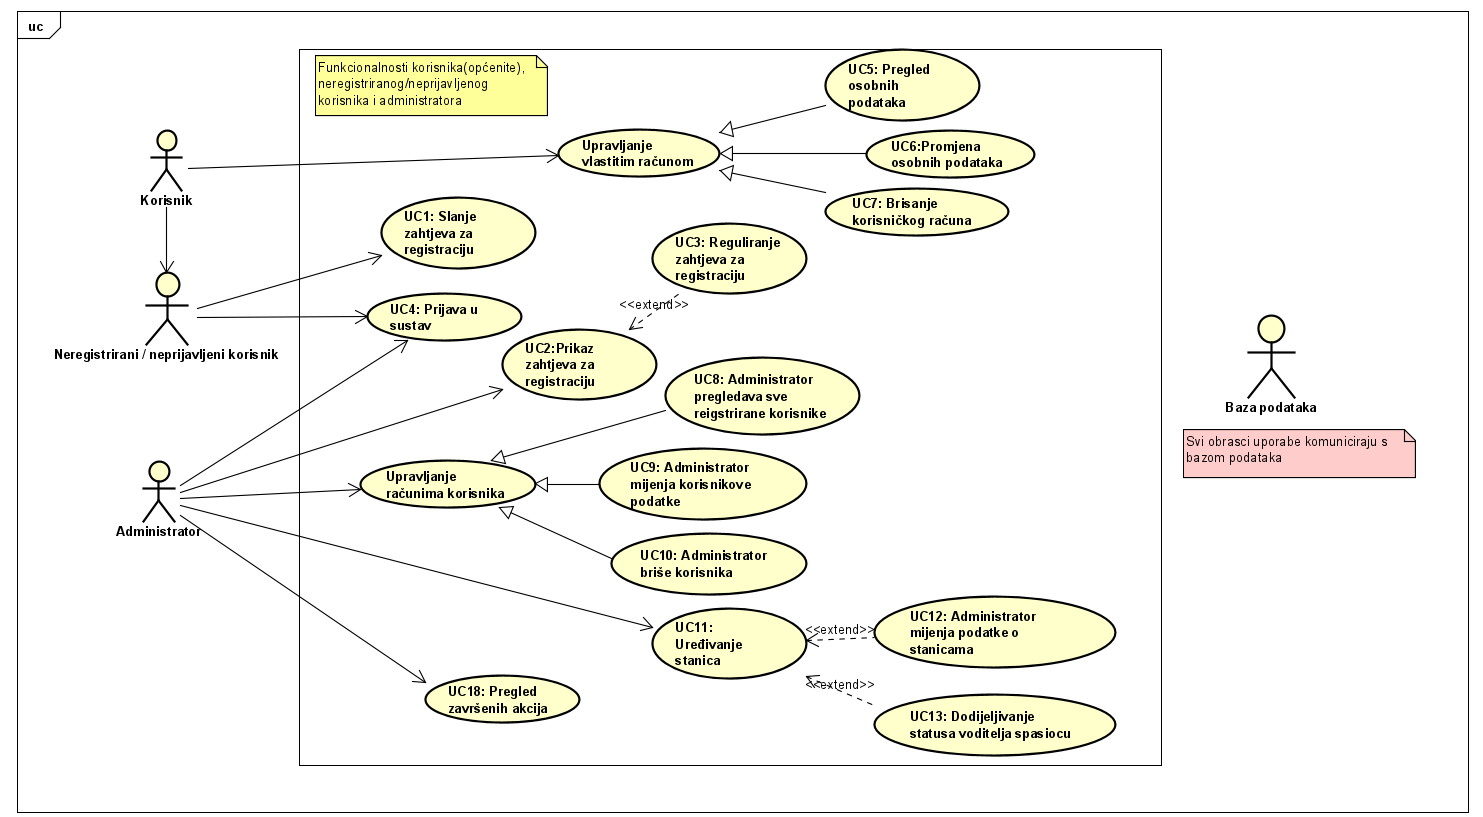
\includegraphics[width=\textwidth]{./slike/Korisnik,Administrator.png}
					\caption{Dijagram obrasca uporabe, funkcionalnost korisnika i administratora}
				
				\end{figure}
				
				\begin{figure}[h!]
					\centering
					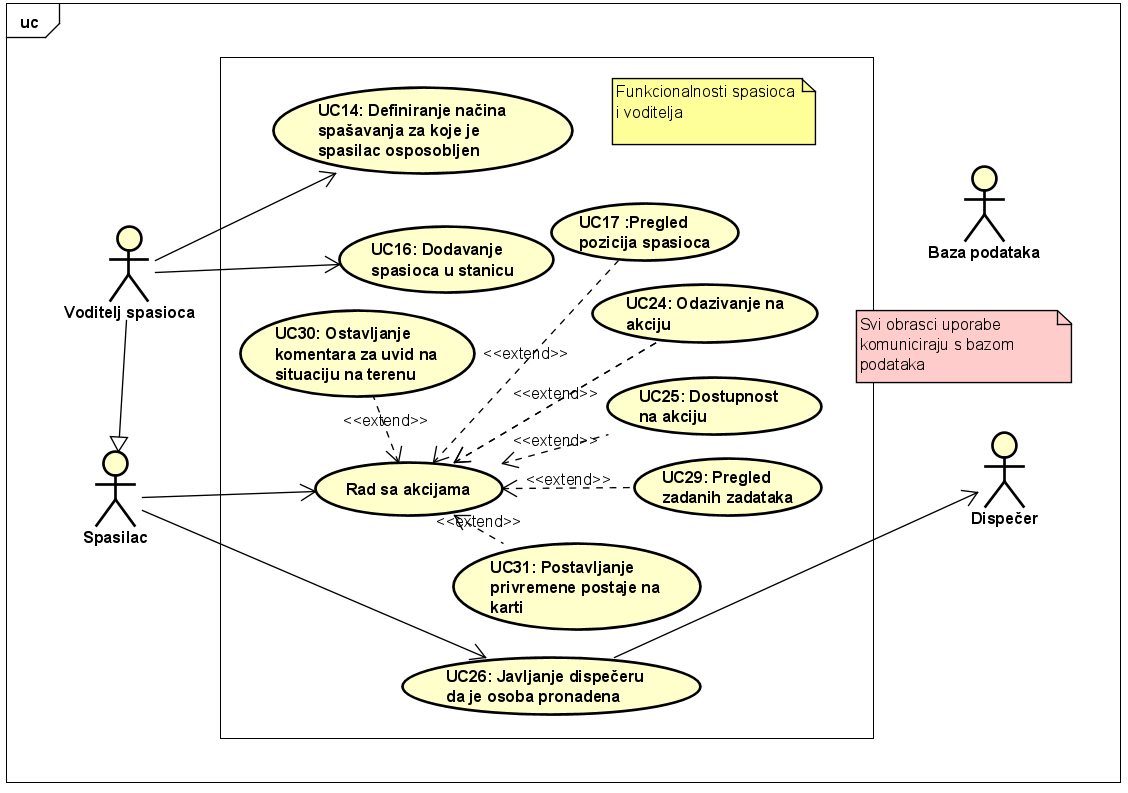
\includegraphics[width=\textwidth]{./slike/Spasioci.png}
					\caption{Dijagram obrasca uporabe, funkcionalnost spasioca}
					
				\end{figure}
				
				\begin{figure}[h!]
					\centering
					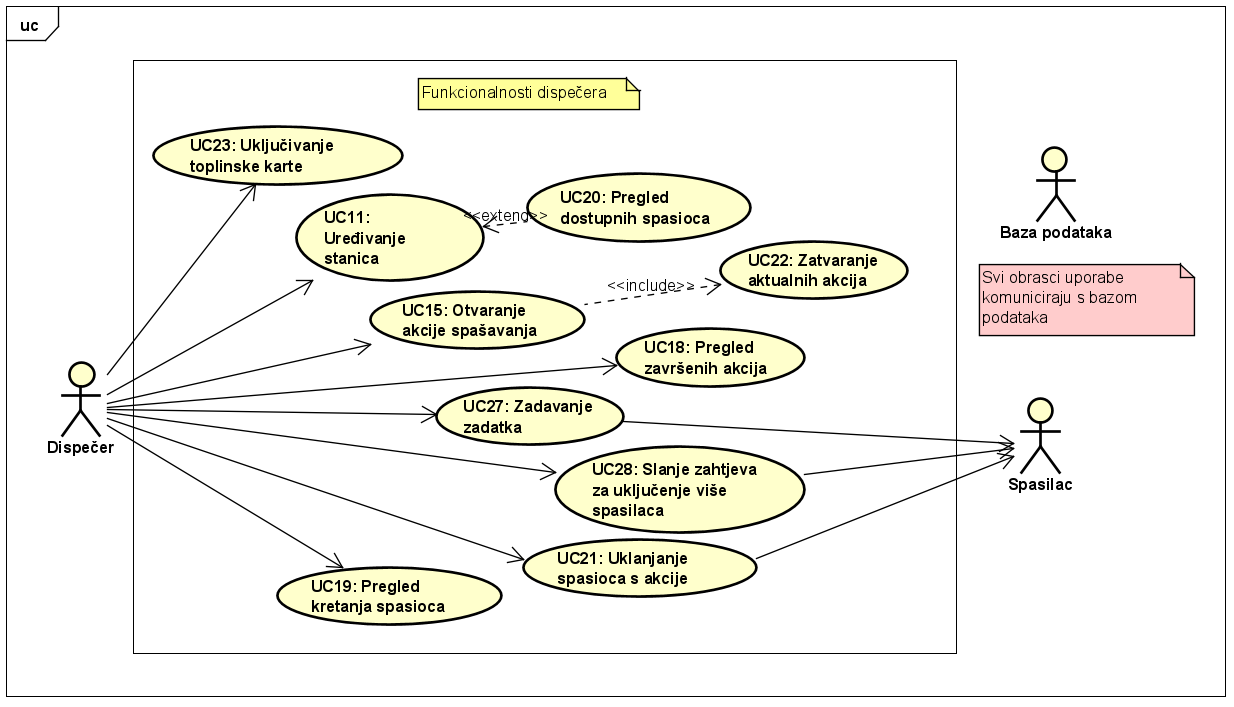
\includegraphics[width=\textwidth]{./slike/Dispecer.png}
					\caption{Dijagram obrasca uporabe, funkcionalnost dispečera}
					
				\end{figure}
			
				\cleardoublepage
				
			\subsection{Sekvencijski dijagrami}
			\begin{packed_item}
				
				
				\item \textbf{Obrazac uporabe UC15 $-$ Otvaranje akcije spašavanja}
				\\
				\item[] \begin{packed_item}
					{Dispečer dobiva poziv za pomoć (vanjska prijava).Upisuje podatke o nestaloj osobi i području na kojem se potraga treba odvijati. Nakon toga, dispečer šalje zahtjev za traženje dostupnih spasilaca čime akcija započinje. Spasioci se ovisno o raspoloživosti javljaju za sudjelovanje u akciji, a dispečer ima pregled svih osoba koje sudjeluju u akciji. U slučaju da se javi prevelik broj spasioca, dispečer ih može (ali ne mora) ukloniti iz akcije. Ako nema dovoljno spasioca, dispečer može poslati zahtjev za uključenje još spasioca u aktivnu akciju spašavanja.}
					
					\begin{figure}[h!]
						\centering
						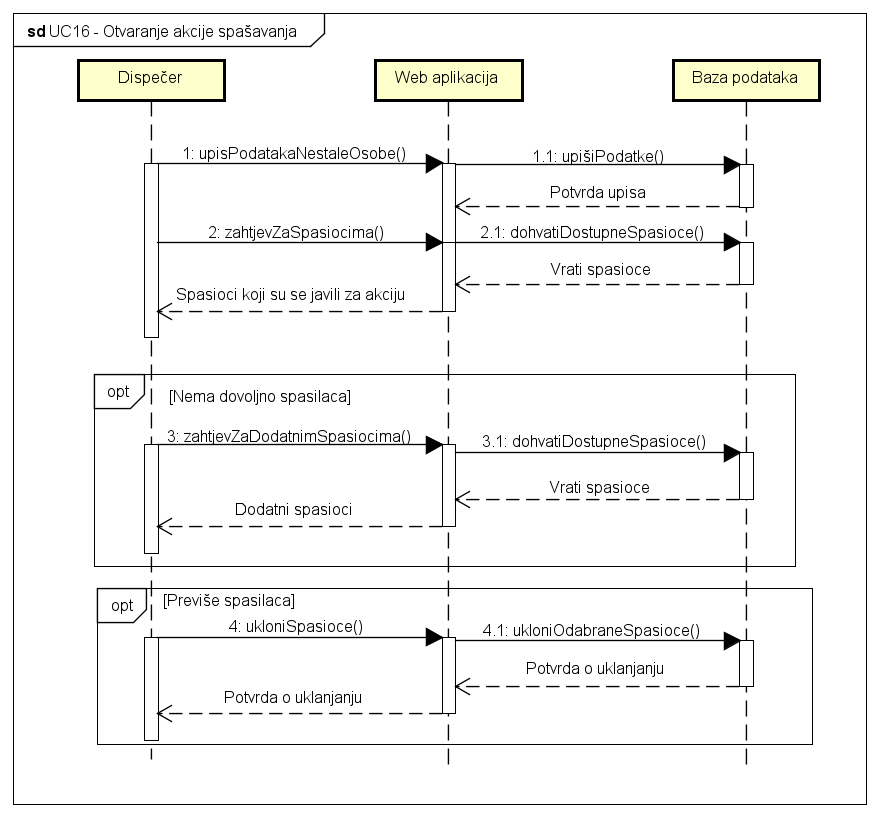
\includegraphics[width=\textwidth]{./slike/UC15.png}
						\caption{Sekvencijski dijagram za UC15}
						
					\end{figure}
					\eject
				\end{packed_item}
				\newpage
					
				\item \textbf{Obrazac uporabe UC24 $-$ Odazivanje na akciju}
				\\
				\item[] \begin{packed_item}
					{Spasilac dobiva obavijest o novoj akciji spašavanja. Ako ima mogućnosti sudjelovati, šalje zahtjev za pridruživanje timu za spašavanje. U slučaju da je osposobljen sudjelovati u toj akciji njegov zahtjev se prihvaća, a u protivnom biva odbijen.Ako je već aktivan na nekoj drugoj akciji, uklanja ga se sa stare akcije i dodaje u željenu akciju spašavanja.}
					
					\begin{figure}[h!]
						\centering
						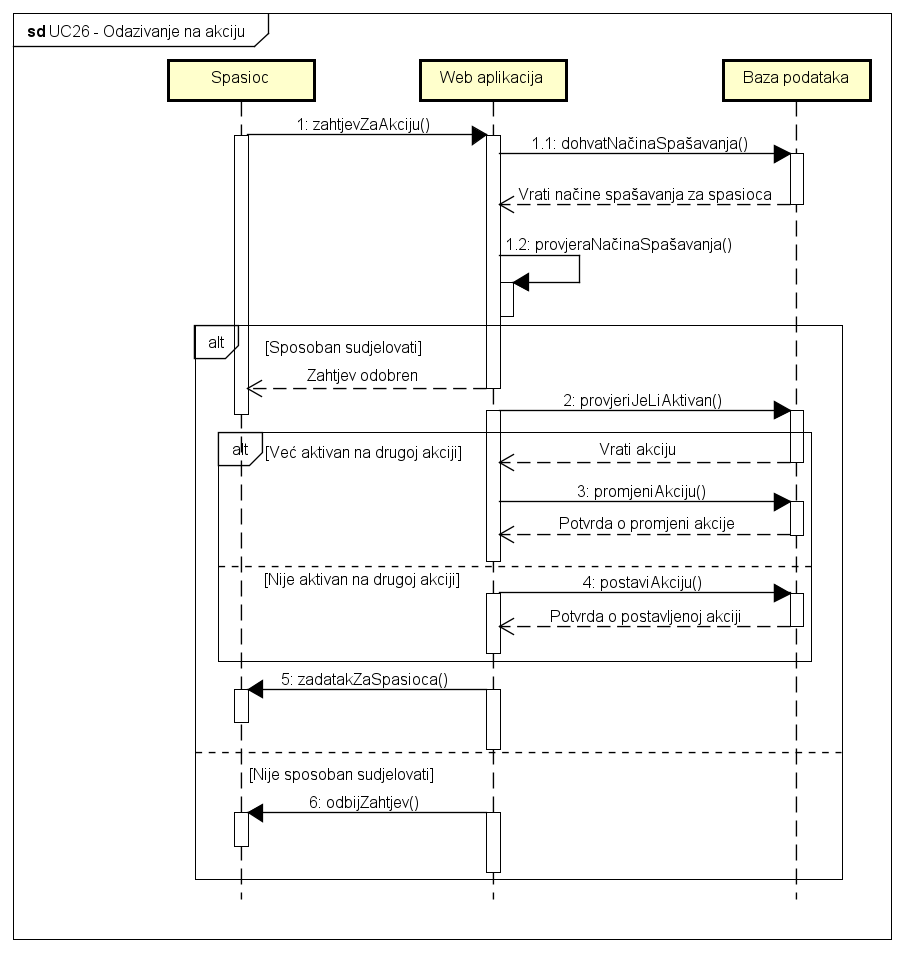
\includegraphics[width=\textwidth]{./slike/UC24.png}
						\caption{Sekvencijski dijagram za UC24}
						
					\end{figure}
					\eject
				\end{packed_item}
				\newpage
					
					
				\item \textbf{Obrazac uporabe UC27 $-$ Zadavanje zadatka}
				\\
				\item[] \begin{packed_item}
					{Dispečer spasiocima na aktivnoj akciji zadaje pojedinačne zadatke. Oni mogu biti: prođi određenom rutom, dođi do lokacije, postavi privremenu postaju ili osvježi zalihe u privremenoj postaji. Ako smatra potrebnim, dispečer može uz zadatak dodati i komentar.}
					
					\begin{figure}[h!]
						\centering
						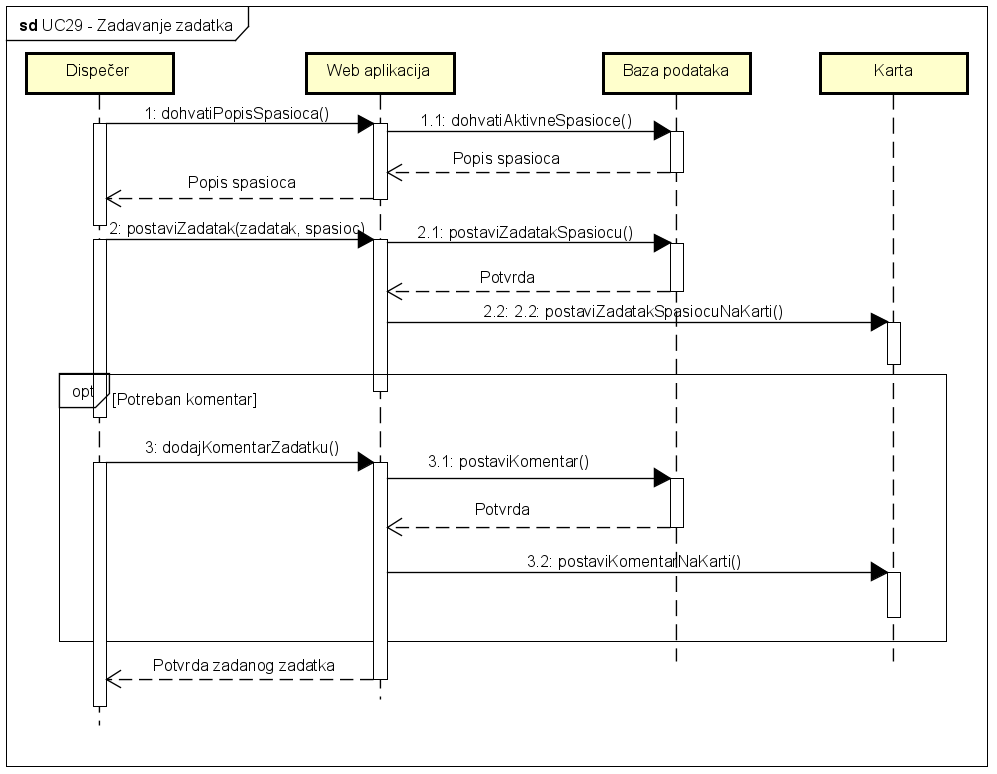
\includegraphics[width=\textwidth]{./slike/UC27.png}
						\caption{Sekvencijski dijagram za UC27}
						
					\end{figure}
					\eject
					
				\end{packed_item}
				\eject
			\end{packed_item}
			\newpage

	
		\section{Ostali zahtjevi\\}
		
		\begin{packed_item}
			
			\item Aplikacija mora omogućiti rad više korisnika u stvarnom vremenu
			\item Korisničko sučelje i sustav moraju podržavati hrvatsku abecedu
			\item Sustav treba biti implementiran kao web aplikacija dostupna svim korisnicima s javnog servisa
			\item Web aplikacija se će biti implementirana koristeći \textit{React} i \textit{Spring Boot framework}
			\item Sustav mora biti lak za održavanje i nadogradnju
			\item Neispravno korištenje aplikacije ne smije narušiti funkcionalnosti i rad sustava
			\item Izvršavanje dijela programa u kojem se pristupa bazi podataka ne smije trajati duže od nekoliko sekundi
			\item Sustav ne smije dozvoliti prikaz informacija korisnicima koji nisu ovlašteni da ih pregledavaju
			\item Sustav ne smije omogućiti korisnicima da obavljaju nedozvoljene operacije nad bazom podataka
			
		\end{packed_item}
			 
			 
			 
	
	\chapter{Arhitektura i dizajn sustava}

	Aplikacija se sastoji od tri podsustava:
	
		\begin{itemize}
			\item Preglednik
			\item Poslužitelj
			\item Baza podataka
		\end{itemize}
	
	Putem preglednika korisnici pristupaju aplikaciji te šalju ili primaju podatke od poslužitelja. Odabrani protokol za komunikaciju između korisnika i aplikacije je HTTP protokol. Za rad na pregledniku odabrana je tehnologija React.
	
	Poslužitelj prihvaća zahtjeve korisnika te šalje informacije nazad na preglednik koji se prikazuju korisniku. Poslužitelj također pristupa bazi podataka te obrađuje podatke koji se nalaze u bazi. Poslužitelj se radi u Java Spring frameworku.
	
	Arhitektura sustava je zasnovana na modelu Model View Component.
	
	
	
	
	
	
	\section{Baza podataka}
		
		
	Odabrana je relacijska baza podataka implementirana pomoću PostgreSQL. Baza podataka je normalizirana te je u trećoj normalnoj formi. Sastavljena je od entiteta
			\begin{itemize}
				\item korisnik
				\item spasilac
				\item dispečer
				\item akcija
				\item stanica
				\item način spašavanja
				\item zadatak
			\end{itemize}
		
			\subsection{Opis tablica}
			
				\begin{longtabu} to \textwidth {|X[7, l]|X[7, l]|X[20, l]|}
					
					\hline \multicolumn{3}{|c|}{\textbf{KORISNIK}}	 \\[3pt] \hline
					\endfirsthead
					
					\hline \multicolumn{3}{|c|}{\textbf{KORISNIK}}	 \\[3pt] \hline
					\endhead
					
					\hline 
					\endlastfoot
					
					\textbf{korisnickoIme} & VARCHAR	&  	Jedinstveno korisničko ime svakog korisnika 	\\ \hline
					lozinka	& VARCHAR & lozinka korisnika	\\ \hline 
					ime & VARCHAR	&  		\\ \hline 
					prezime & VARCHAR & \\ \hline
					brojMob & VARCHAR & broj mobitela korisnika \\ \hline
					email & VARCHAR & email korisnika \\ \hline
					uloga & VARCHAR & varijabla koja služi u backend dijelu za dodjeljivanje u određenu tablicu(spasilac/dispečer) \\ \hline
					status & VARCHAR & status je li korisnik registriran ili nije \\ \hline
					
					
				\end{longtabu}
				
				\begin{longtabu} to \textwidth {|X[7, l]|X[7, l]|X[20, l]|}
					
					\hline \multicolumn{3}{|c|}{\textbf{DISPEČER}}	 \\[3pt] \hline
					\endfirsthead
					
					\hline \multicolumn{3}{|c|}{\textbf{DISPEČER}}	 \\[3pt] \hline
					\endhead
					
					\hline 
					\endlastfoot
					
					\textbf{korisnickoIme} & VARCHAR	&  	Ujedno i strani ključ na tablicu korisnik, u tablici se spremaju svi korisnici koji su dispečeri 	\\ \hline
					
					
				\end{longtabu}
				
				\begin{longtabu} to \textwidth {|X[7, l]|X[7, l]|X[20, l]|}
					
					\hline \multicolumn{3}{|c|}{\textbf{SPASILAC}}	 \\[3pt] \hline
					\endfirsthead
					
					\hline \multicolumn{3}{|c|}{\textbf{SPASILAC}}	 \\[3pt] \hline
					\endhead
					
					\hline 
					\endlastfoot
					
					\textbf{korisnickoIme} & VARCHAR	&  	Ujedno i strani ključ na tablicu korisnik, u tablici se spremaju svi korisnici koji su spasioci 	\\ \hline
					\textit{sifStanica} & VARCHAR & Šifra stanice kojoj pripada spasilac \\ \hline
					dostupan & BOOLEAN & Je li spasilac dostupan za odazivanje na akciju \\ \hline
					
				\end{longtabu}
				
				\begin{longtabu} to \textwidth {|X[7, l]|X[7, l]|X[20, l]|}
					
					\hline \multicolumn{3}{|c|}{\textbf{STANICA}}	 \\[3pt] \hline
					\endfirsthead
					
					\hline \multicolumn{3}{|c|}{\textbf{STANICA}}	 \\[3pt] \hline
					\endhead
					
					\hline 
					\endlastfoot
					
					\textbf{sifStanica} & VARCHAR	&  	Jedinstvena šifra stanice 	\\ \hline
					nazivStanica & VARCHAR & Ime stanice \\ \hline
					\textit{korImeVoditelj} & VARCHAR & Korisničko ime spasioca koji je voditelj stanice \\ \hline
					
				\end{longtabu}
				
				\begin{longtabu} to \textwidth {|X[7, l]|X[7, l]|X[20, l]|}
					
					\hline \multicolumn{3}{|c|}{\textbf{AKCIJA}}	 \\[3pt] \hline
					\endfirsthead
					
					\hline \multicolumn{3}{|c|}{\textbf{AKCIJA}}	 \\[3pt] \hline
					\endhead
					
					\hline 
					\endlastfoot
					
					\textbf{sifAkcija} & VARCHAR	&  	Jedinstvena šifra akcije 	\\ \hline
					nazivAkcija & VARCHAR & Ime akcije \\ \hline
					infNestalaOsoba & VARCHAR & Kratki opis i informacije o nestaloj osobi \\ \hline
					lokacija & VARCHAR & Lokacija potrage \\ \hline
					\textit{korImeDispečer} & VARCHAR & Dispečer koji koordinira akciju \\ \hline
					status & VARCHAR & Status akcije (u tijeku/završena) \\ \hline
					
				\end{longtabu}
				
				\begin{longtabu} to \textwidth {|X[7, l]|X[7, l]|X[20, l]|}
					
					\hline \multicolumn{3}{|c|}{\textbf{ZADATAK}}	 \\[3pt] \hline
					\endfirsthead
					
					\hline \multicolumn{3}{|c|}{\textbf{ZADATAK}}	 \\[3pt] \hline
					\endhead
					
					\hline 
					\endlastfoot
					
					\textbf{sifZadatak} & VARCHAR & Jedinstvena šifra zadatka \\ \hline
					nazivZadatak & VARCHAR & Naziv zadatka \\ \hline
					\textit{korImeDispecer} & VARCHAR & Dispečer koji je spasiocu zadao zadatak \\ \hline
					\textit{korImeSpasilac} & VARCHAR & Spasilac kojem je zadan zadatak \\ \hline
					komentar & VARCHAR & Komentar za određeni zadatak \\ \hline
					
					
				\end{longtabu}
				
				\begin{longtabu} to \textwidth {|X[7, l]|X[7, l]|X[20, l]|}
					
					\hline \multicolumn{3}{|c|}{\textbf{SPASILACAKCIJA}}	 \\[3pt] \hline
					\endfirsthead
					
					\hline \multicolumn{3}{|c|}{\textbf{SPASILACAKCIJA}}	 \\[3pt] \hline
					\endhead
					
					\hline 
					\endlastfoot
					
					\textbf{korImeSpasilac} & VARCHAR & Korisničko ime spasioca na određenoj akciji \\ \hline
					\textit{sifAkcija} & VARCHAR & Šifra akcije na kojoj sudjeluje određeni spasilac
					
					
				\end{longtabu}
				
				\begin{longtabu} to \textwidth {|X[7, l]|X[7, l]|X[20, l]|}
					
					\hline \multicolumn{3}{|c|}{\textbf{SPASILACAKCIJA}}	 \\[3pt] \hline
					\endfirsthead
					
					\hline \multicolumn{3}{|c|}{\textbf{SPASILACAKCIJA}}	 \\[3pt] \hline
					\endhead
					
					\hline 
					\endlastfoot
					
					\textbf{korImeSpasilac} & VARCHAR & Korisničko ime spasioca na određenoj akciji \\ \hline
					\textit{sifAkcija} & VARCHAR & Šifra akcije na kojoj sudjeluje određeni spasilac 
					
					
				\end{longtabu}
			
				\begin{longtabu} to \textwidth {|X[7, l]|X[7, l]|X[20, l]|}
					
					\hline \multicolumn{3}{|c|}{\textbf{NACINSPASAVANJA}}	 \\[3pt] \hline
					\endfirsthead
					
					\hline \multicolumn{3}{|c|}{\textbf{NACINSPASAVANJA}}	 \\[3pt] \hline
					\endhead
					
					\hline 
					\endlastfoot
					
					\textbf{sifNacin} & VARCHAR & Šifra načina spašavanja \\ \hline
					imeNacin & VARCHAR & Naziv načina spašavanja \\ \hline
					intenzitet & INT & Kolikim intenzitetom se može tragati s ovakvim načinom \\ \hline
					velicina & INT & Koliko područje se može pretražiti s ovakvim načinom	\\ \hline			 	
					
					
				\end{longtabu}
			
				\begin{longtabu} to \textwidth {|X[7, l]|X[7, l]|X[20, l]|}
					
					\hline \multicolumn{3}{|c|}{\textbf{ZAHTJEV}}	 \\[3pt] \hline
					\endfirsthead
					
					\hline \multicolumn{3}{|c|}{\textbf{ZAHTJEV}}	 \\[3pt] \hline
					\endhead
					
					\hline 
					\endlastfoot
					
					\textbf{sifAkcija} & VARCHAR & Korisničko ime spasioca na određenoj akciji \\ \hline
					\textbf{sifStanica} & VARCHAR & Šifra akcije na kojoj sudjeluje određeni spasilac \\ \hline
					\textit{sifNacin} & VARCHAR & Način spašavanja koji se zahtijeva od određene stanice \\ \hline
					
				\end{longtabu}
			
				\begin{longtabu} to \textwidth {|X[7, l]|X[7, l]|X[20, l]|}
					
					\hline \multicolumn{3}{|c|}{\textbf{SPASILACNACIN}}	 \\[3pt] \hline
					\endfirsthead
					
					\hline \multicolumn{3}{|c|}{\textbf{SPASILAC}}	 \\[3pt] \hline
					\endhead
					
					\hline 
					\endlastfoot
					
					\textbf{korImeSpasilac} & VARCHAR & Korisničko ime spasioca na određenoj akciji \\ \hline
					\textbf{sifNacin} & VARCHAR & Šifra načina na koje sve može određeni spasilac sudjelovati u akciji \\ \hline
					
					
				\end{longtabu}
		
		\subsection{Dijagram baze podataka}
		\begin{figure}[h!]
			\centering
			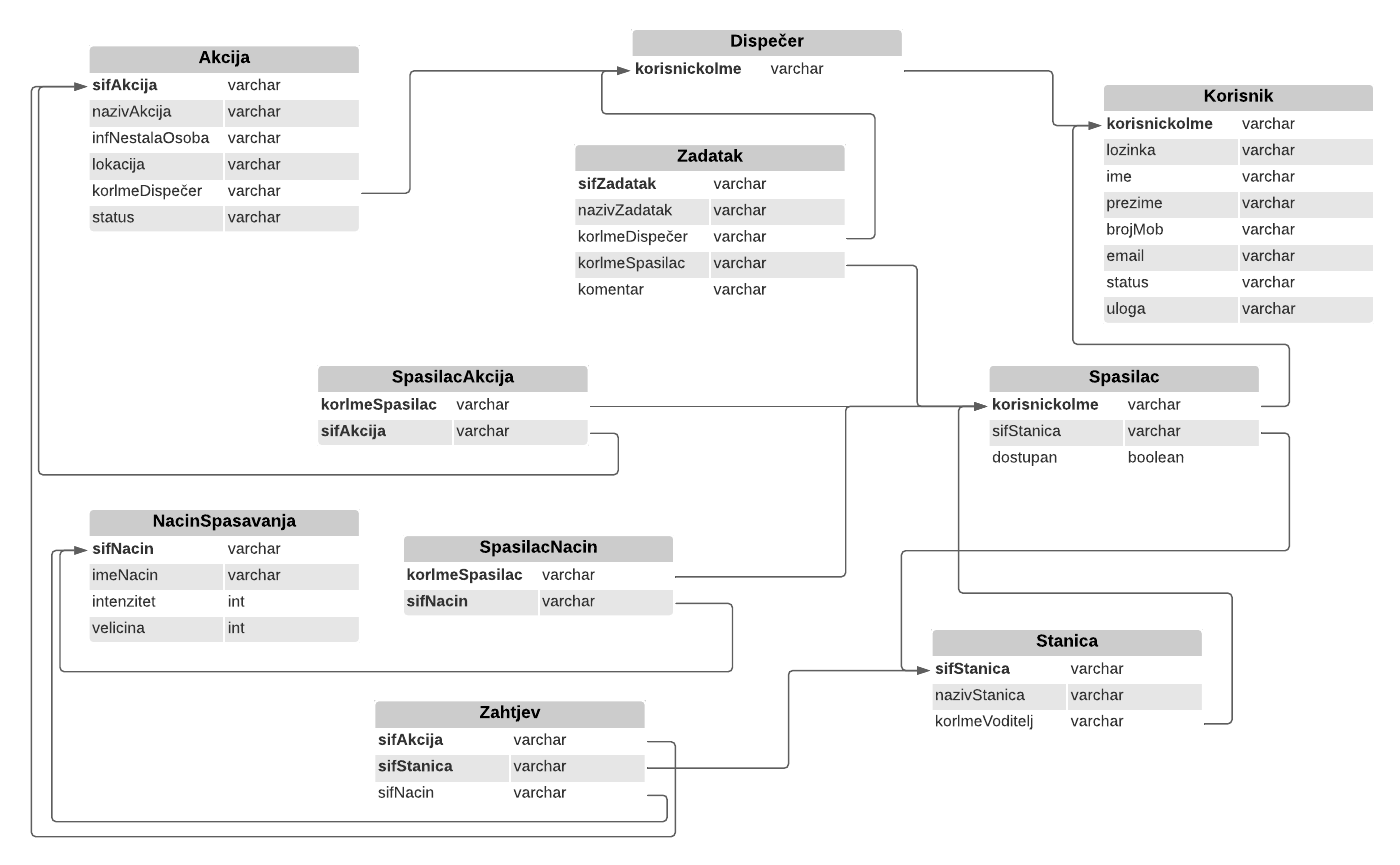
\includegraphics[width=\textwidth]{./slike/dijagrambaze.png}
			\caption{Dijagram baze podataka}
			
		\end{figure}
		
		\eject
	
	
	\section{Dijagram razreda\\}
	
	
	{Na priloženim slikama moguće je vidjeti dijagrame razreda \textit{backend} dijela MVC \\arhitekture.\\}
	
	
	{Na slici 4.2 je prikazana \textbf{Application Controller} klasa  koja se sastoji od metoda koje koriste metode iz \textbf{KorisnikDao}  klase, koja  služi za pristup podataka iz baze sustava.Klasi KorisnikDao controller  pristupa preko funkcija iz \textbf{KorisnikService} klase}\\
	
	\begin{figure}[h!]
		\centering
		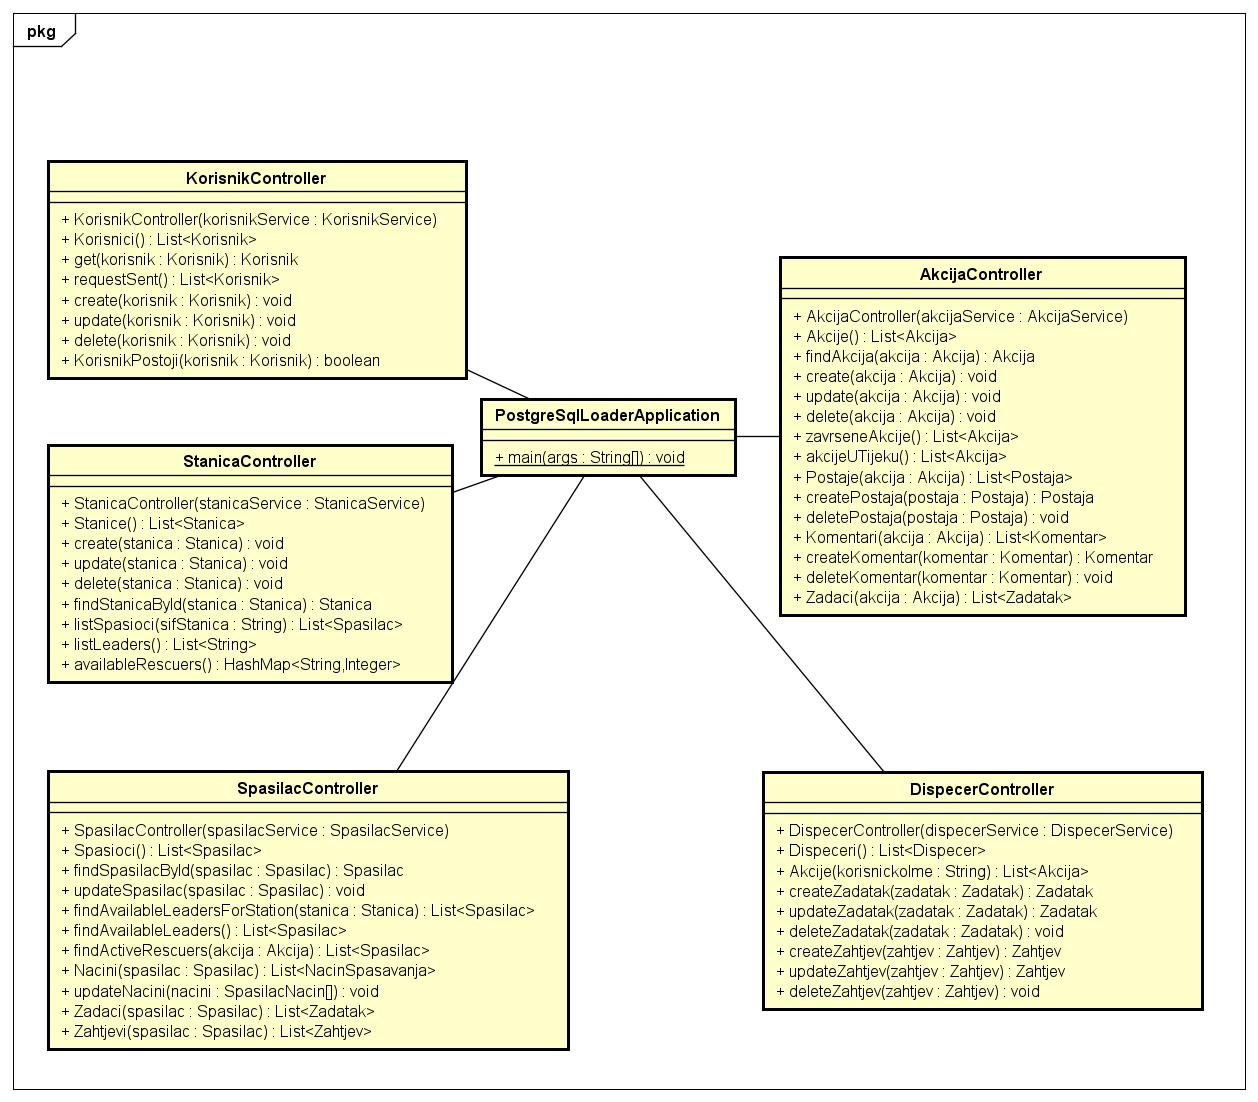
\includegraphics[width = \linewidth]{./slike/Controllers.jpg}
		\caption{Prikaz klase AplicationController}
		
	\end{figure}
	\newpage
	
	{Slika 4.3 prikazuje klase \textbf{Service} te klase \textbf{ServiceImpl} }
	{koje služe za prikaz entiteta kroz bazu za manipuliranje podatcima.\newline Slika također prikazuje ovisnost Sve ove klase se služe klasom entiteta istog imena koja omogućuje prikaz te manipulaciju s podatcima iz baze podataka.\\}\\
	
	\begin{figure}[h!]
		\centering
		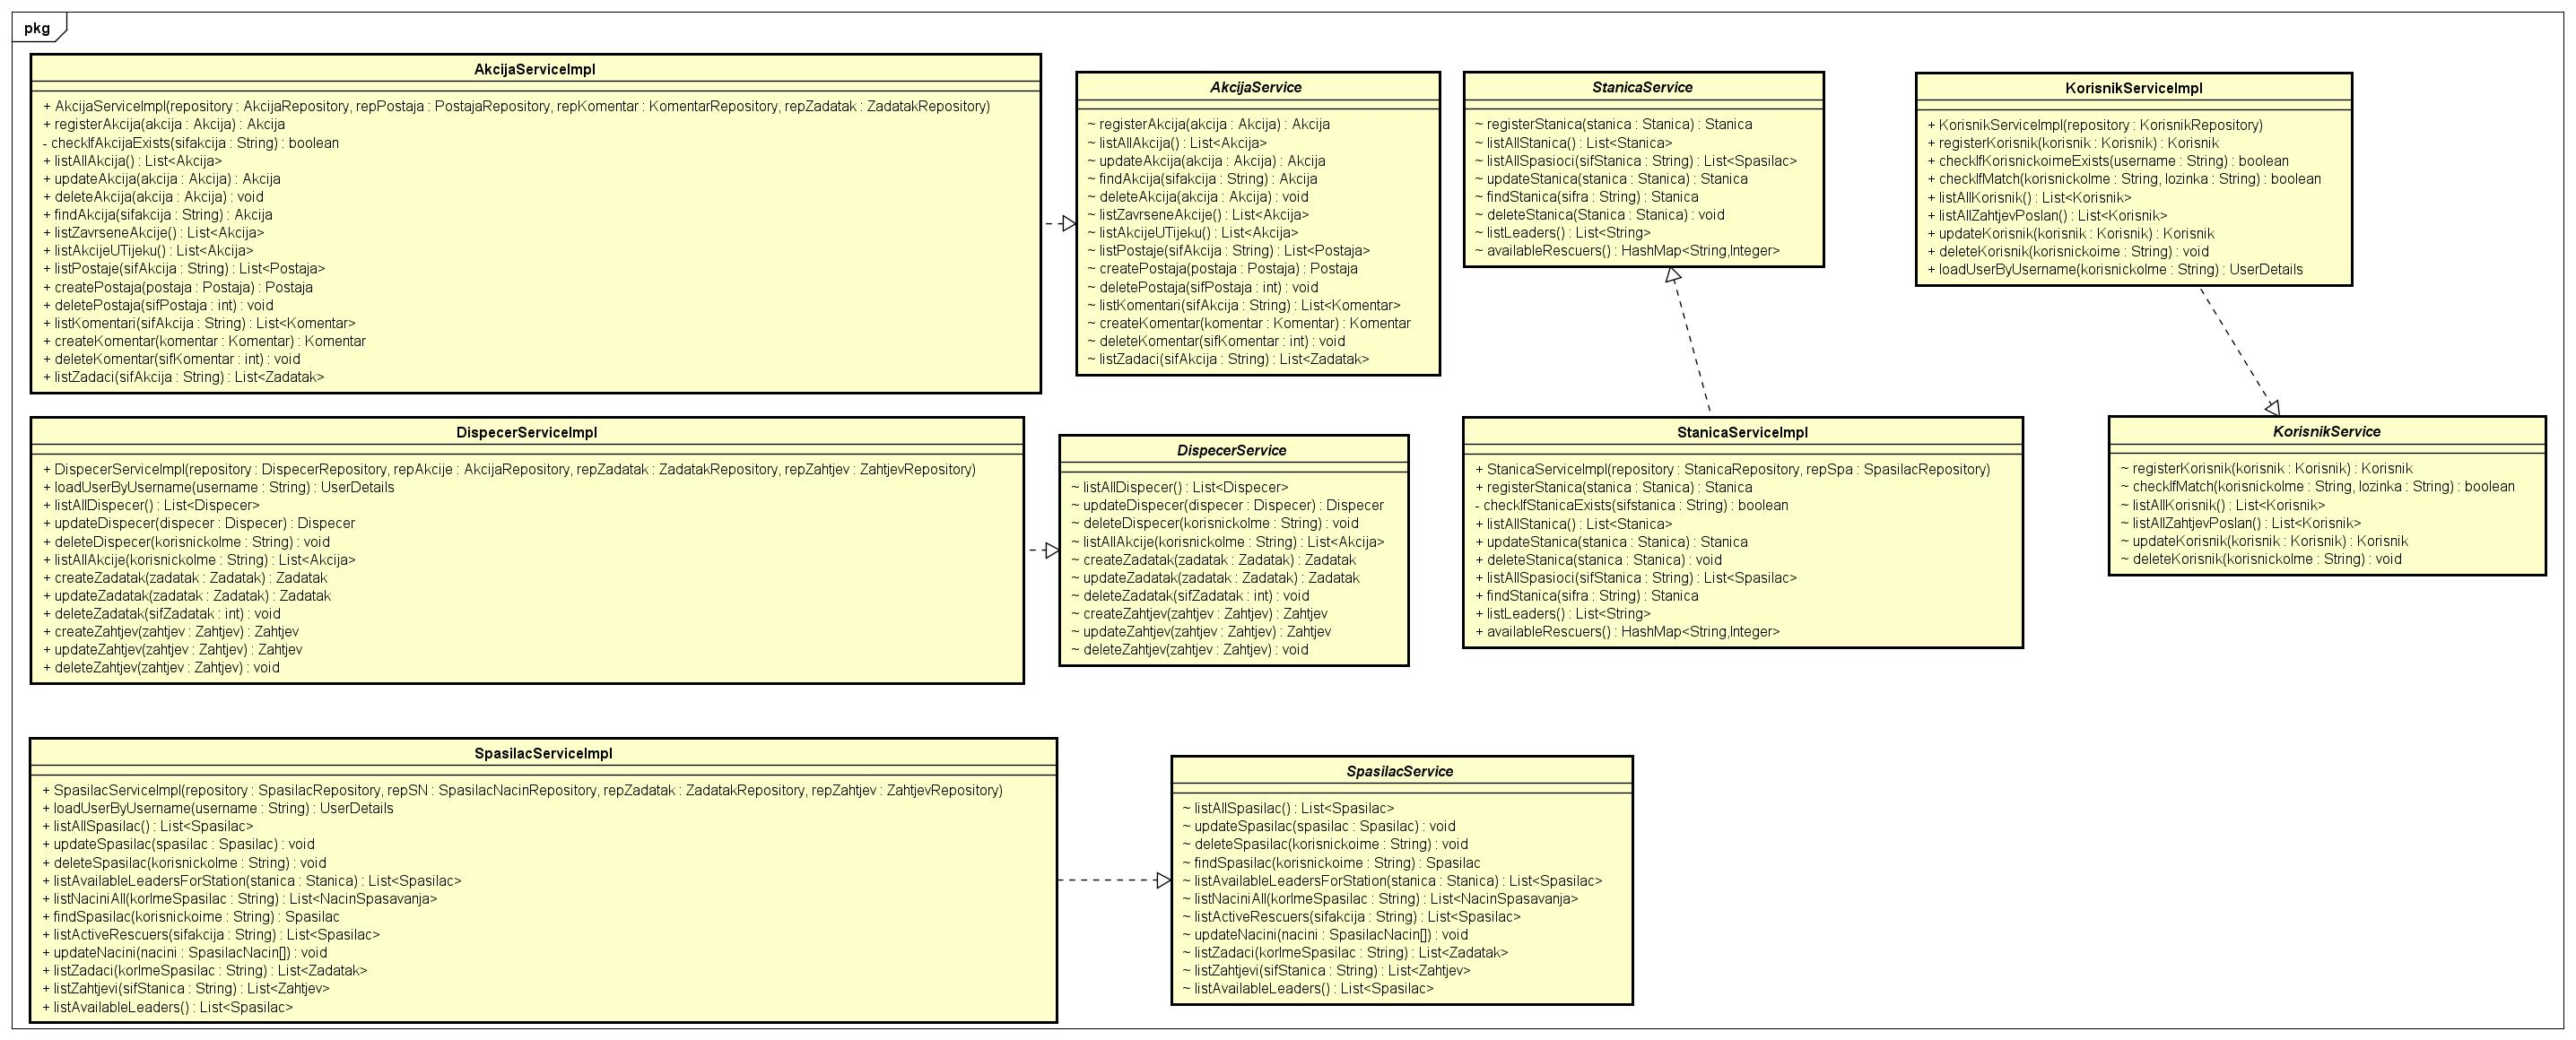
\includegraphics[width=\linewidth]{./slike/ServisImpl.jpg}
		\caption{Prikaz klasa servisa te klasa vezanih uz njihovu implementaciju}
		
	\end{figure}	
	\newpage
	{Za pristup bazi podataka te podatcima u njoj koriste se klase \textbf{Entity} koje koriste \textbf{JPA} funkcije za manipuliranje podataka. Na temelju entitet klasa u kojima podatci moraju biti navedeni istim redoslijedom kao i u bazi podataka funkcije pretražuju podatke.Entiteti aplikacije prikazani su na slici 4.4\\}
	
	\begin{figure}[h!]
		\centering
		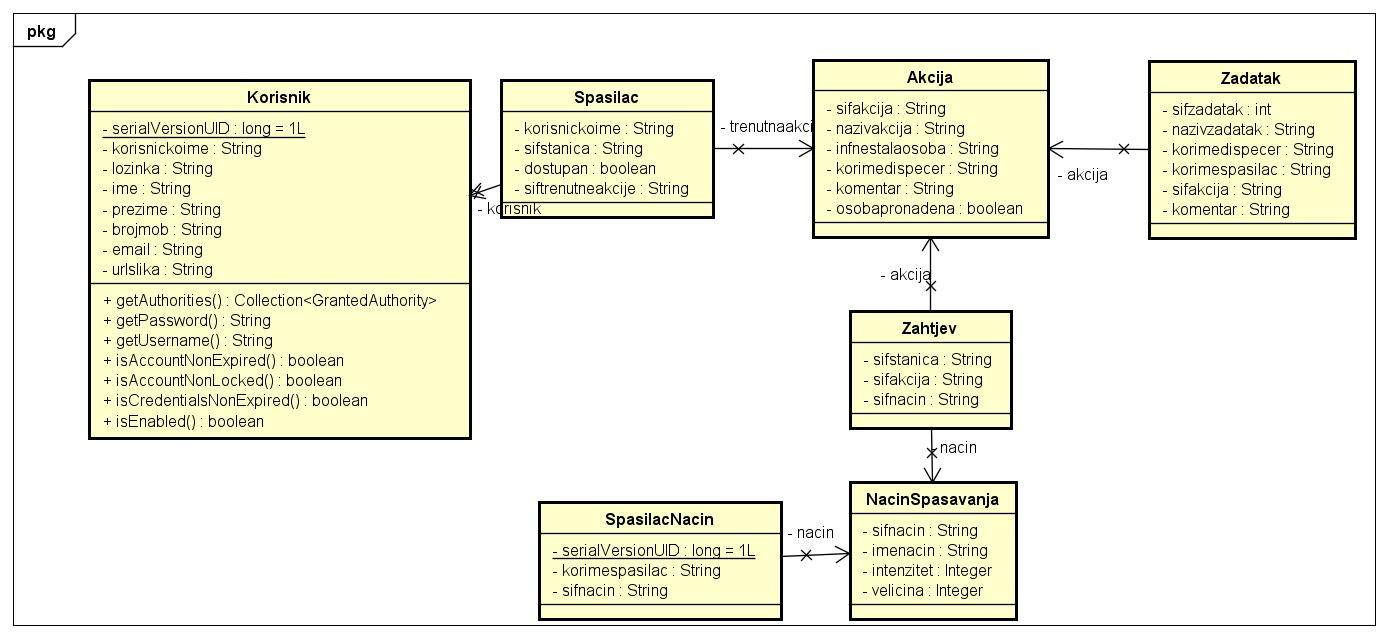
\includegraphics[width=\linewidth]{./slike/Entiteti.jpg}
		\caption{Prikaz klasa Entiteta koji su apstraktni prikazi podataka u bazi podataka}
		
	\end{figure}

	\eject
	
	\newpage
	\section{Dijagram stanja}
	
		{Dijagram stanja prikazuje stanja objekta te prijelaze iz jednog stanja u drugo temeljene na događajima. Na slici 4.5 prikazan je dijagram stanja za spasioca čiji su podatci prethodno potvrđeni od strane admina. Pri prijavi spasiocu se prikazuje početna stranica iz koje može prijeći na neko od drugih stanja(dijelova aplikacije). Za karticu "Trenutna akcija" spasilac može ostaviti komentare na akciju, postaviti privremenu postaju, te javiti dispečeru da je tražena žrtva pronađena. Za karticu "Akcije u tijeku" spasilac može vidjeti koje su trenutačno aktivne akcije na koje se može dobrovoljno prijaviti. Spasilac također ima i mogućnost vidjeti jesu li mu poslani zahtjevi za prijavu na neku od akcija,gumb "Pregled zahtjeva za spasioce",gdje su zahtjevi slani od strane dispečera ili voditelja stanice spasioca. Klikom na "Profil" spasilac ima mogućnost mijenjanja vlastitih osobnih podataka, brisanja svojega računa ako nema potrebu ili ne želi koristiti aplikaciju u budućnosti te javljanja svojeg trenutnog stanja (dostupnost za akcije).}
	
		\begin{figure}[h!]
			\centering
			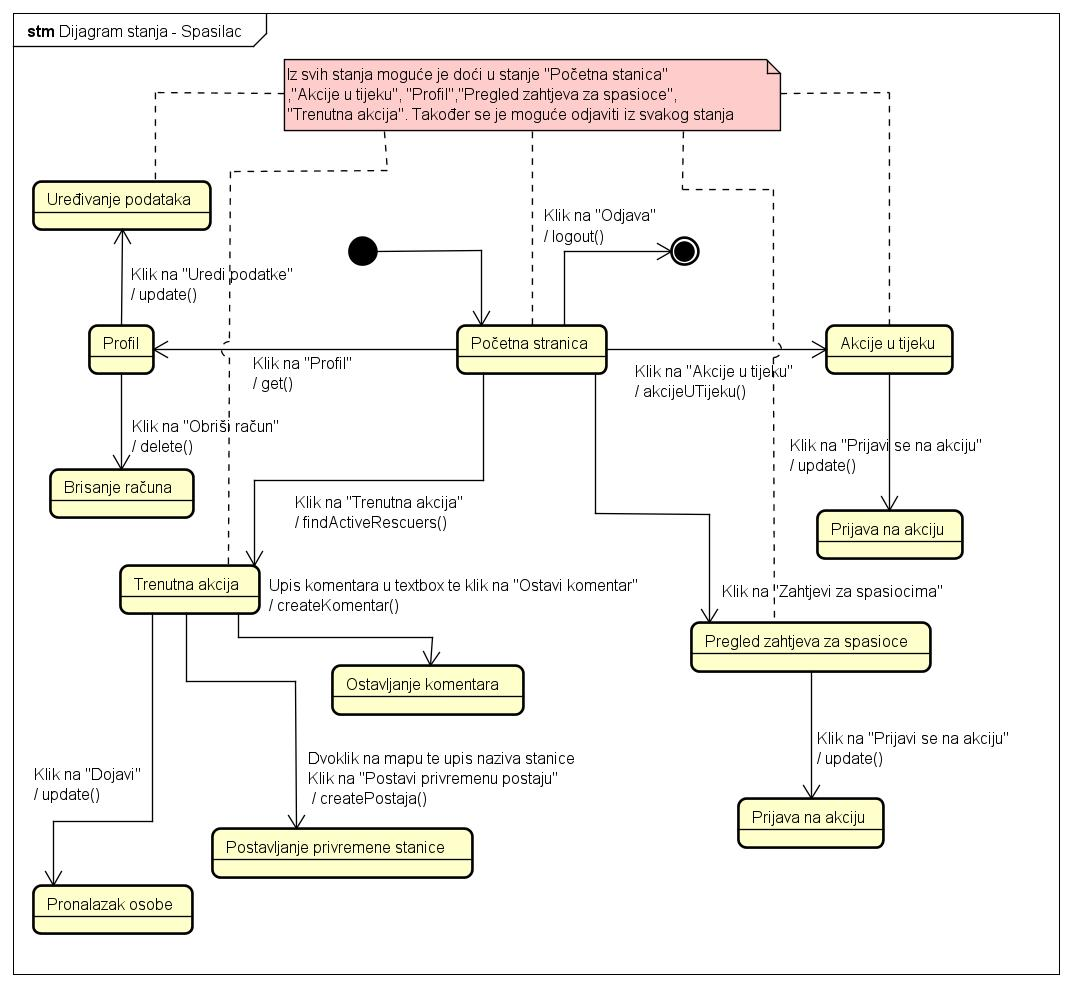
\includegraphics[width=\linewidth]{./slike/Dijagram stanja - Spasilac.jpg}
			\caption{Prikaz dijagrama stanja}
		
		\end{figure}
	
	
	\eject 
	
	\section{Dijagram aktivnosti}
	
 	\begin{packed_item}
		\item	{Dijagram aktivnosti primjenjuje se za opis modela toka upravljanja ili toka podataka za pregled na aplikaciji. U modeliranju toka upravljanja svaki korak obavlja se nakon završetka koraka koji mu prethodi s naglaskom na jednostavnost. Na dolje prikazanim dijagramima (slike 4.6 i 4.7) prikazani su razni procesi koje aplikacija izvodi ovisno o traženim upitima korisnika.\\
			Slika 4.6 prikazuje proces javljanja spasioca na akciju. Korisnik se prijavi u sustav, potom izabire jednu od trenutno aktivnih akcija spašavanja te klikom na gumb se prijavljuje u istu}
		
		\begin{figure}[h!]
			\centering
			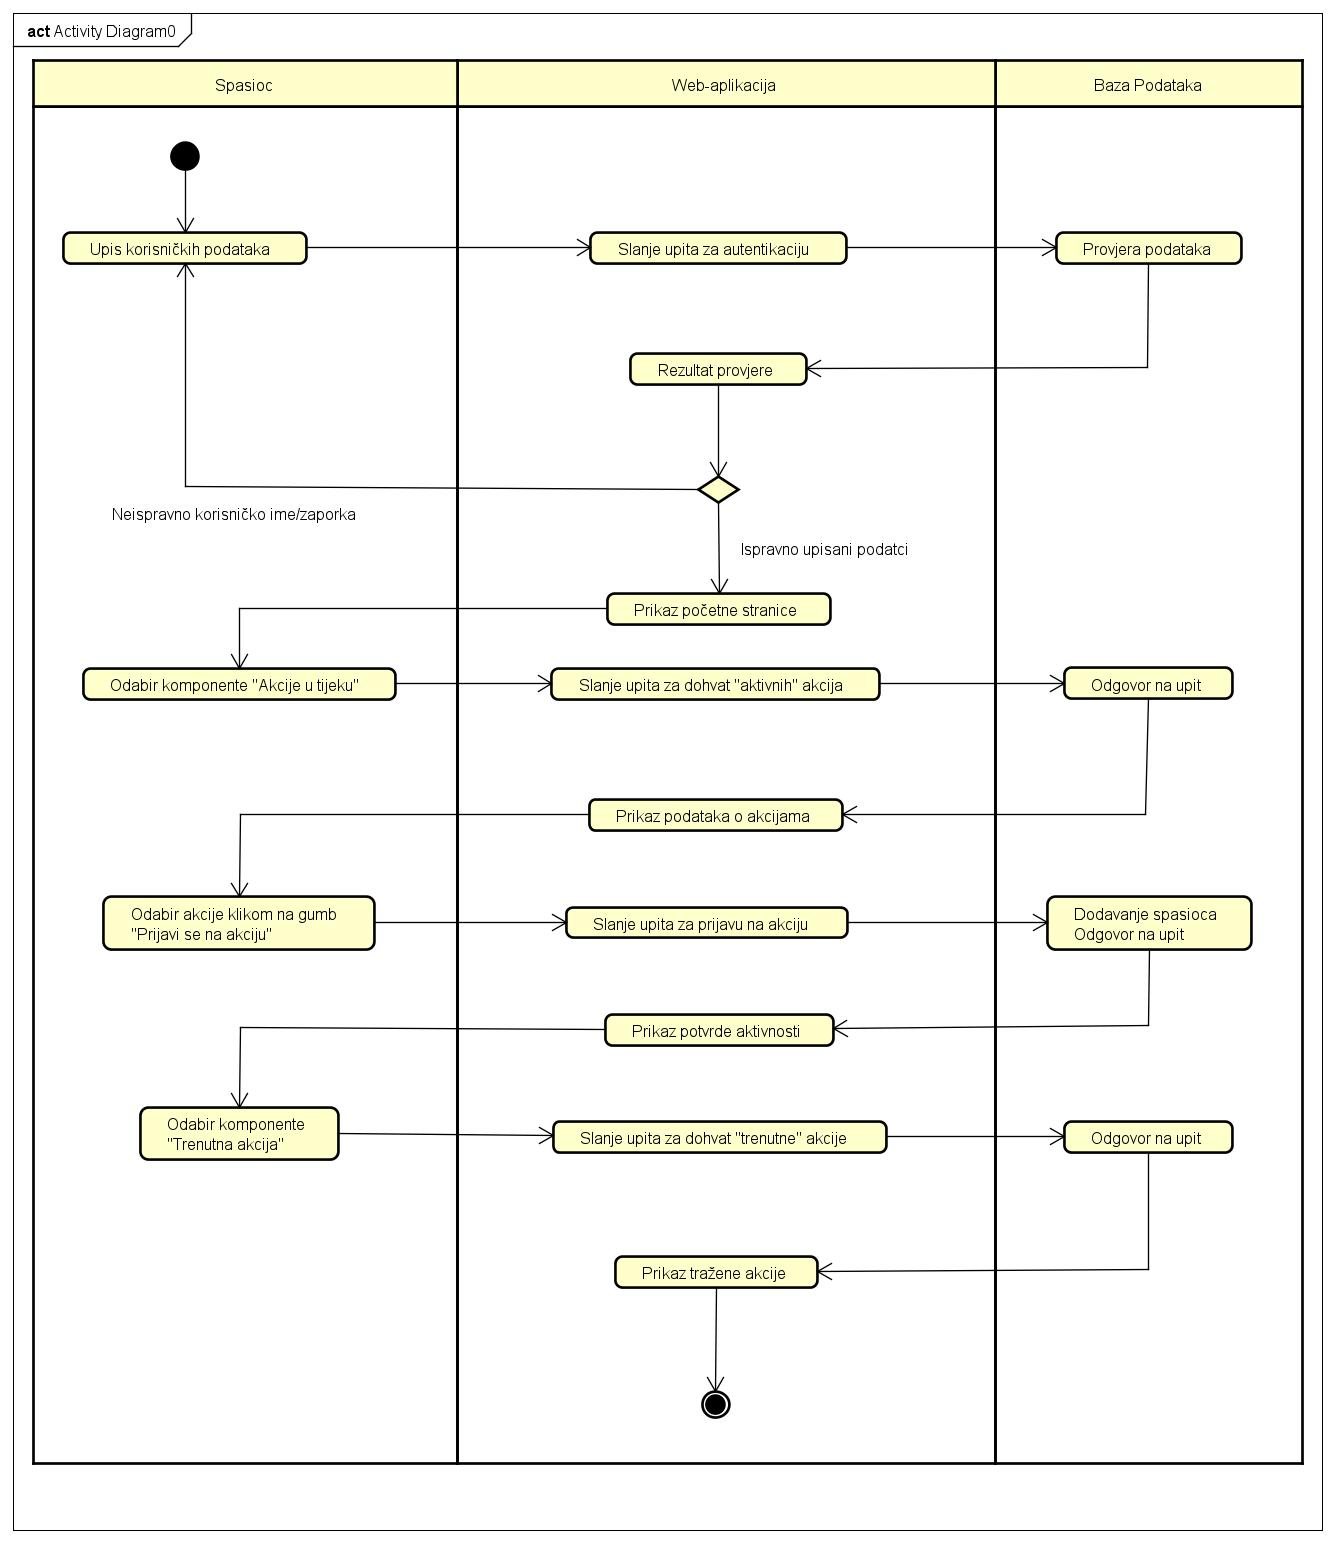
\includegraphics[width=\linewidth]{./slike/PrijavaNaAkciju.jpg}
			\caption{Prikaz dijagrama aktivnosti za javljanje spasioca na akciju}
			
		\end{figure}
		\eject
		
	\end{packed_item}
		\newpage
		\begin{packed_item}
			\begin{figure}[h!]
				
				\centering
				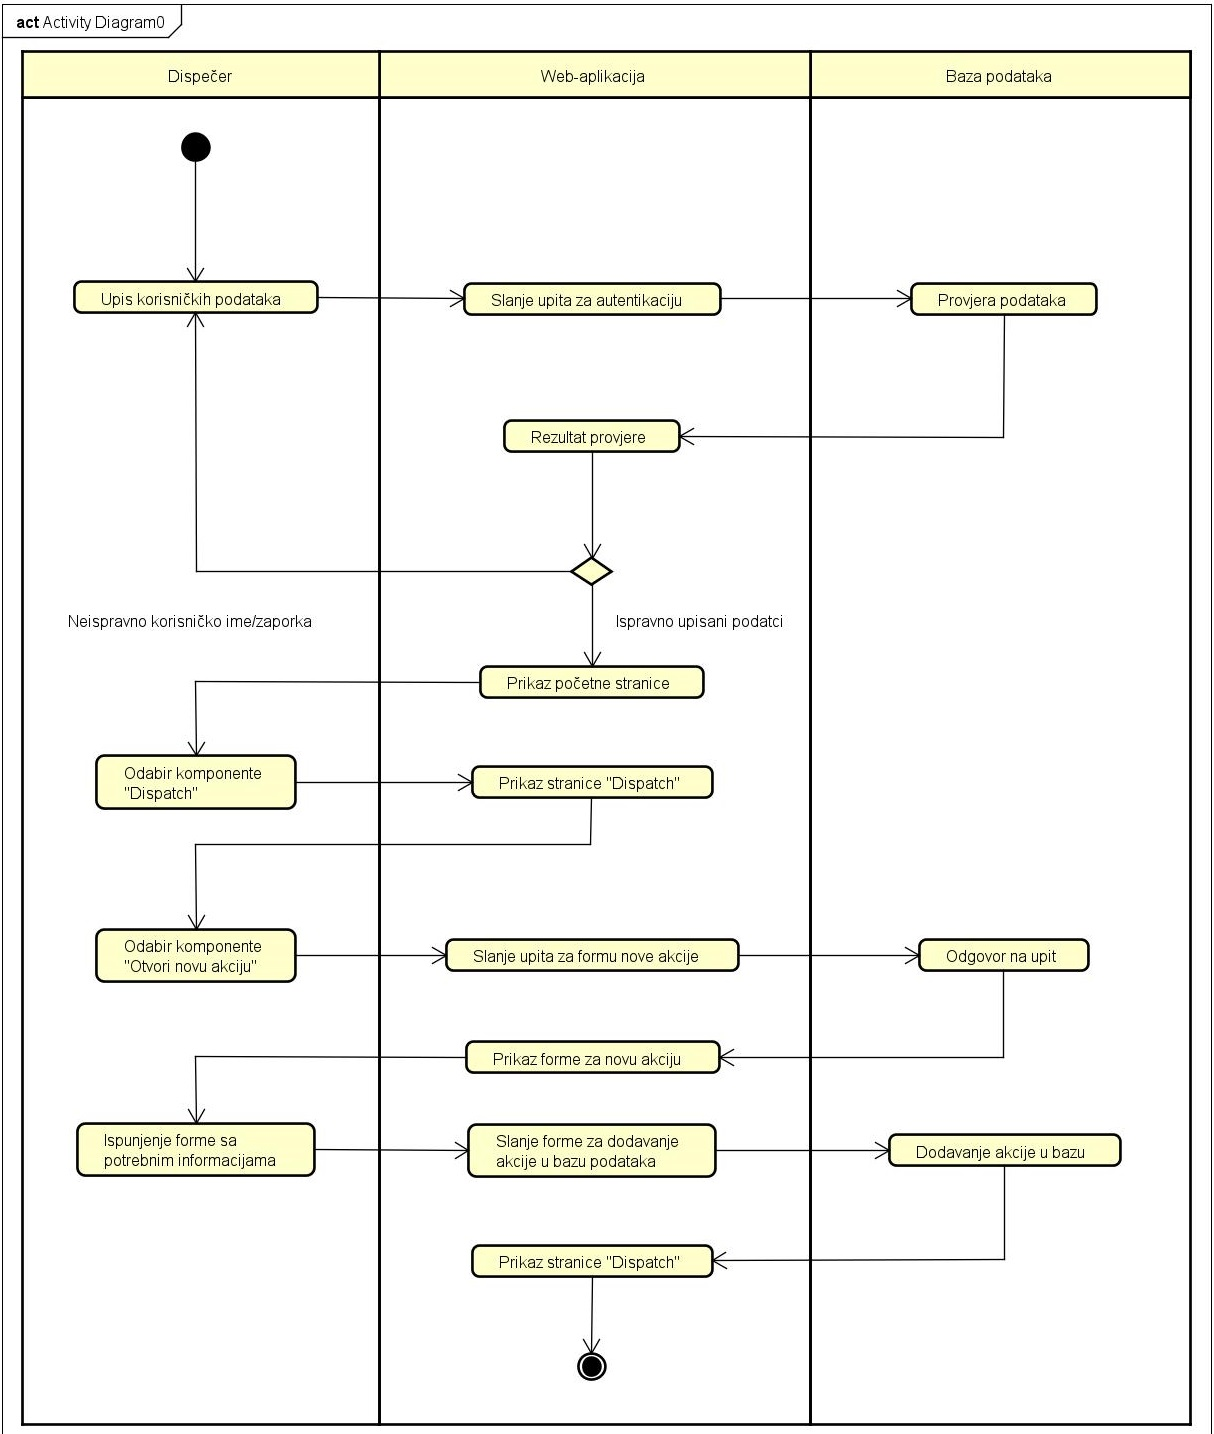
\includegraphics[width=\linewidth]{./slike/StvaranjeAkcije.jpg}
				\caption{Prikaz dijagrama aktivnosti za stvaranje nove akcije spašavanja}
			\end{figure}
			\eject
			
			\item {Slika 4.7 prikazuje proces stvaranja nove akcije spašavanja.Dispečer je dužan otvoriti karticu dispatch te klikom na gumb "Otvori novu akciju". Zatim mu se na upit šalje forma za ispunu informacija o novoj akciji i osobi. Pri završetku ispune forme akcija je dodana u bazu podataka te je dispečer vraćen na stranicu Dispatch.}\\
			
			
		\end{packed_item}
	\newpage

	\section{Dijagram komponenti}
	

		{Dijagram komponenti prikazan na slici dolje(slike 4.8) prikazuje organizaciju i međuovisnost komponenti, unutarnje strukture te odnose komponenata prema njihovoj okolini.Web-aplikaciji se pristupa pomoću dva sučelja. Koristimo sučelje za dohvat HTML,CSS i JS datoteka dobivamo datoteke vezane za \textit{frontend} dio aplikacije.Router je komponenta aplikacije koja na upis podataka ovisno o razini dozvola određuje koja datoteka će biti poslužena korisniku na sučelju. Svaki dio \textit{frontend} arhitekture raspoređen je u nekolicine JavaScript datoteka koje su raspodijeljene u logičke cjeline, neke od kojih su nazvane po kategoriji korisnika koji postoje u aplikaciji. Sve datoteke u našem projektu koje su oblika JavaScript ovise o \textbf{REACT} biblioteci preko koje dohvaćaju razne komponente potrebne za ispravan rad aplikacije,npr. gumbi,forme i sl.Preko sučelja \textbf{REST API} dohvaćaju se datoteke tipa JSON. \textbf{REST API} koristi za posluživanje \textit{backend} dijela podataka. Za poslugu podataka iz baze podataka koristi se \textbf{JPA} oblik podataka u datotekama te za upite u bazu.React-view komponenta pomoću svih navedenih sučelja komunicira za \textit{HGSSTracks} aplikacijom i s naputkom korisnikovih akcija na samoj aplikaciji osvježava prikaz ,prikazuje nove podatke koje je korisnik zatražio ili datoteke tj. upite koje je korisnik slao a vezane su za bazu podataka.}\\
		
		\begin{figure}[h!]
			\centering
			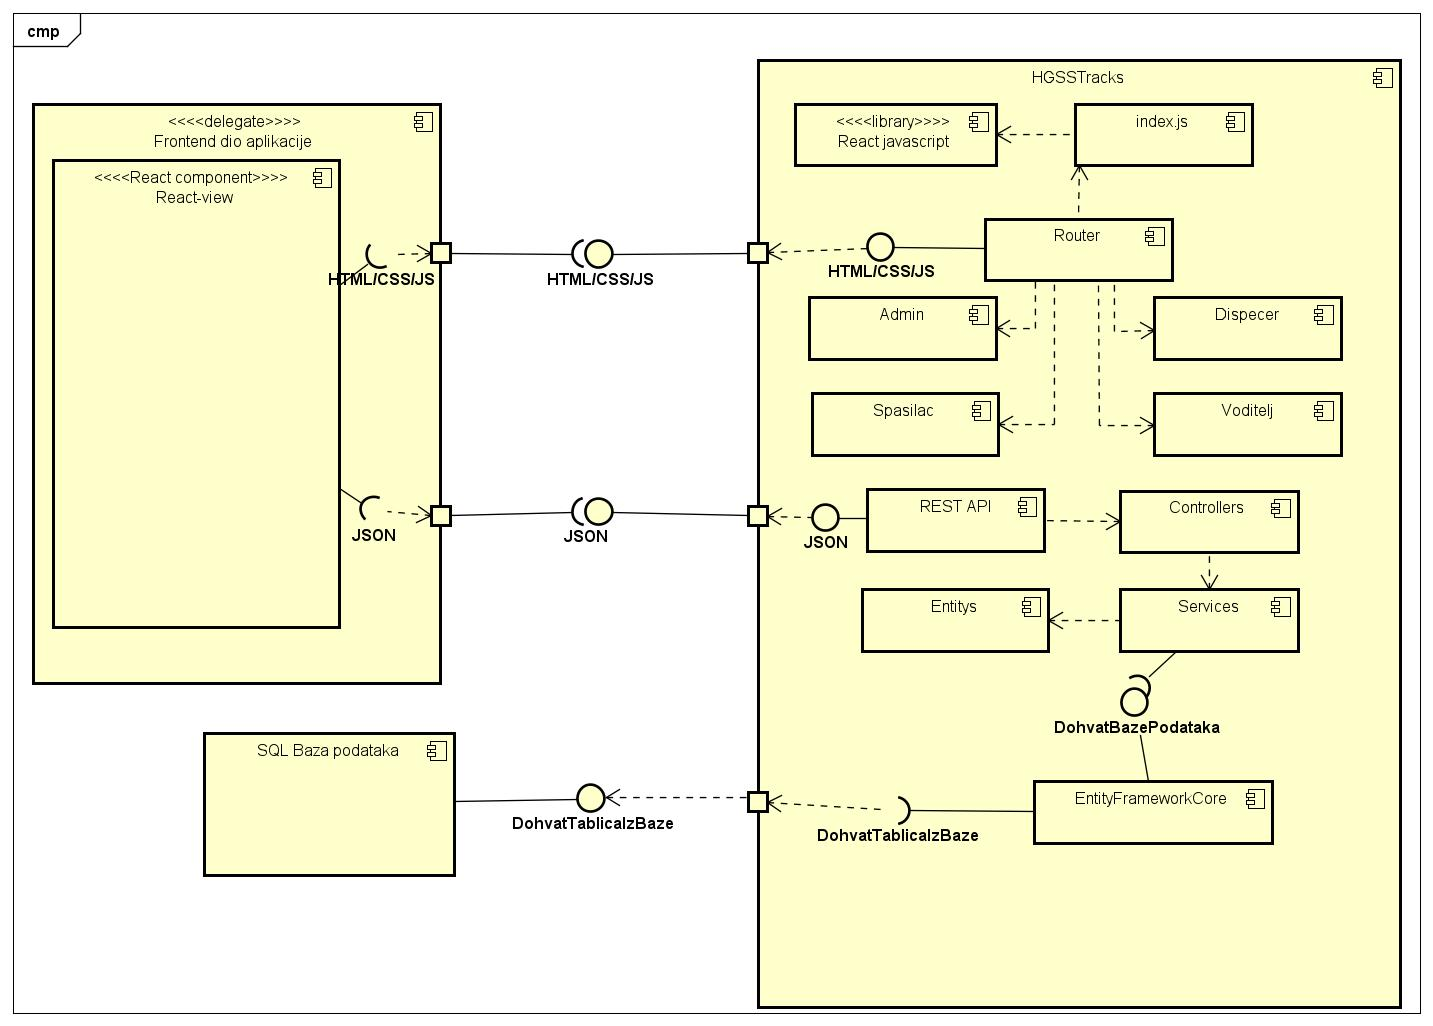
\includegraphics[width=\linewidth]{./slike/DijagramKomponenti.jpg}
			\caption{Prikaz dijagrama komponenti}
			
		\end{figure}
	\chapter{Implementacija i korisničko sučelje}
		
		
		\section{Korištene tehnologije i alati}
		

			
			 	{U projektu smo koristili različita razvojna okruženja i alate za svaku granu projekta.\\
			 	Za izradu i rad na bazi podataka korišten je alat \textbf{\href{https://www.pgadmin.org/}{pgAdmin}} za rad s \textbf{\href{https://www.postgresql.org/}{PostgreSQL}} tehnologijom,koji je omogućavao lakše praćenje stanje baze i povijest provedenih traženja i postavki u bazi\\
			 	Za \textit{backend} dio projekt korišteno je razvojno okruženje \textbf{\href{https://www.eclipse.org/}{Eclipse}} u kojem je program pisan \textbf{\href{https://www.java.com/en/}{Java}} programskim jezikom sa \textbf{\href{https://spring.io/projects/spring-boot}{Spring boot}} radni okvir sa znatnim programskim kraticama i nadogradnjama, te \textbf{\href{https://maven.apache.org/}{Maven}} podrškom za dohvaćanja programskih ovisnosti u projektu\\
			 	Za \textit{frontend} je korišteno razvojno okruženje \textbf{\href{https://code.visualstudio.com/}{Visual studio code}} u kojem je dodajući ekstenzije bio omogućen bolji rad s tehnologijom \textbf{\href{https://reactjs.org/}{REACT}} koja je znatno ubrzala rad na izgledu i funkcionalnosti stranice prikazane korisniku.
			 	\textbf{\href{https://nodejs.org/en/}{Node.js}} je služio za upravljanjem ostalih programskih ovisnosti u Reactu. \textbf{\href{https://leafletjs.com/}{Leaflet}}-om se dobivaju podaci o karti, a \textbf{\href{http://project-osrm.org/}{OSRM}} za traži put između lokacija.\\
			 	Za međusobno dijeljene koda korištena je tehnologija \textbf{\href{http://www.git-scm.com/}{Git}} te udaljeni repozitorij \textbf{\href{https://about.gitlab.com/}{GitLab}} za svima dostupnu pohranu.\\
			 	Komunikacija pri radu je ostvarena \textbf{\href{https://www.whatsapp.com/}{WhatsApp}} mobilnom aplikacijom za dogovaranje termina i raspodjele obaveza,te \textbf{\href{https://discord.com/}{Discord}} programom za glasovnu komunikaciju pri timskom radu.\\
			 	Za dokumentaciju korišten je alat \textbf{\href{https://tug.org/texlive/}{TexStudio}} u kombinaciji sa TexLive programom koji je generirao PDF dokumente iz .tex datoteka.\\
			 	Za izradu UML dijagrama koristili smo alat \textbf{\href{https://astah.net/}{Astah}} koji smo dobili na korištenje studentskom licencom}.
			
			
			\eject 
		
	\newpage
		\section{Ispitivanje programskog rješenja}
			

			
			{U sljedećem potpoglavlju ispitivanje funkcionalnosti sustava izvedeno je korištenjem ekstenzije za web preglednik "Chrome" pod imenom "Selenium IDE".}
	
			
			\subsection{Ispitivanje komponenti}
			{Pri ispitivanju komponenti ispitani su Obrasci uporabe \textbf{UC1} do \textbf{UC7}. U nastavku su dani kodovi ispitivanja osnovnih funkcionalnih zahtjeva naše aplikacije.}
			
			\newpage
			\begin{packed_item}
				\item {Prikaz koda s kojim je ispitano slanje registracije novog korisnika.}\\
				
				\begin{figure}[h!]
					\centering
					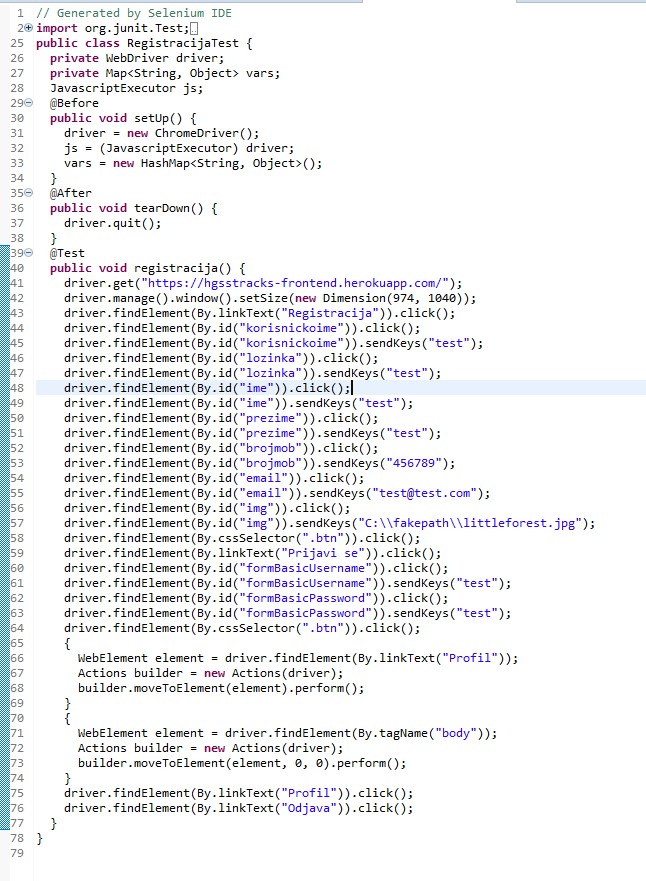
\includegraphics[width=\linewidth]{./slike/TestRegistracije.jpg}
					\caption{Prikaz koda ispitivanja UC1}
				\end{figure}
				\eject
			\end{packed_item}
		
			\newpage
			\begin{packed_item}
				\item {Prikaz koda u kojemu je ispitivan pokušaj prijave u sustav s profilom koji nije bio odobren od strane jednog od admina aplikacije (dodatna mjera sigurnosti).}\\
				
				\begin{figure}[h!]
					\centering
					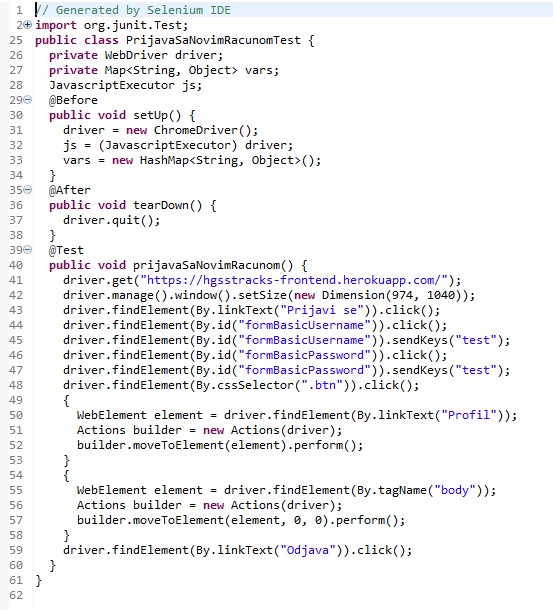
\includegraphics[width=\linewidth]{./slike/PokusajPrijaveSaNepotvdrenimRacunom.jpg}
					\caption{Prikaz koda ispitivanja \textbf{UC4} s kredencijama koje nisu potvrđene od strane admina}
				\end{figure}
				\eject
			\end{packed_item}
		
			\newpage
			\begin{packed_item}
				\item {Prijava u račun jednog od admina te pregled zahtjeva za registraciju i prihvaćanje istog.}\\
				
				\begin{figure}[h!]
					\centering
					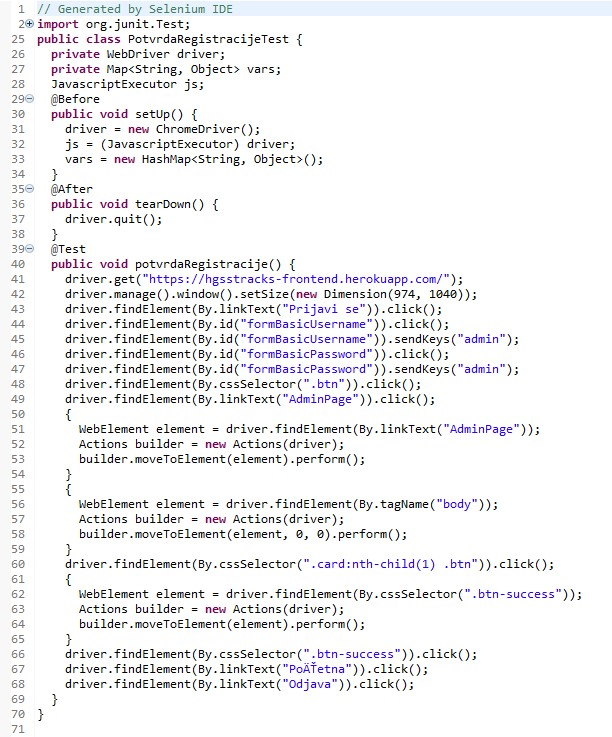
\includegraphics[width=\linewidth]{./slike/ManipulacijaRegistracija.jpg}
					\caption{Prikaz koda ispitivanja \textbf{UC2} i \textbf{UC3}}
				\end{figure}
				\eject
			\end{packed_item}
		
			\newpage
			\begin{packed_item}
				\item {Prijava s novo nastalim profilom (također potvrđenim) te mijenjanje informacija o korisniku, u ovom slučaju izvedena je promjena telefonskog broja spasioca.}\\
				
				\begin{figure}[h!]
					\centering
					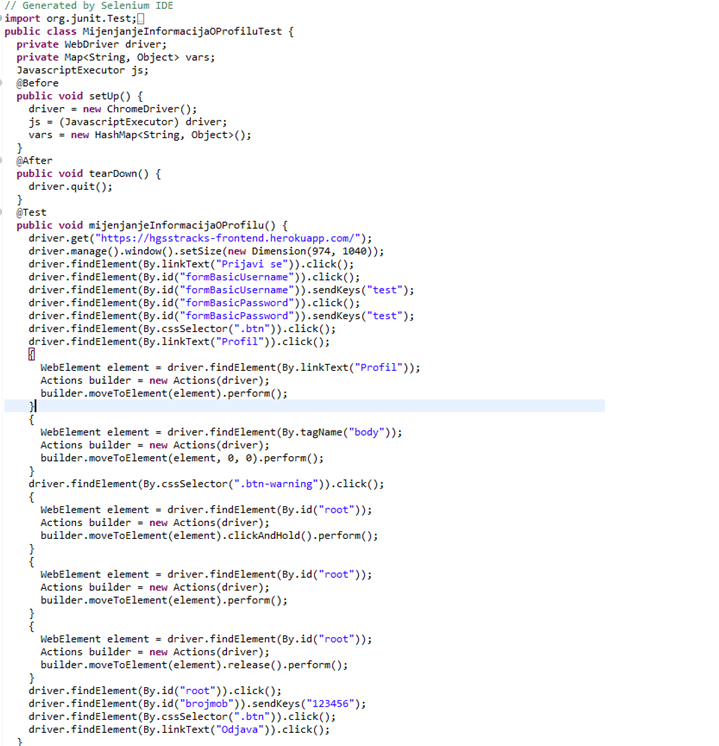
\includegraphics[width=\linewidth]{./slike/Slika2.png}
					\caption{Prikaz koda ispitivanja \textbf{UC4, UC5} i \textbf{UC6}}
				\end{figure}
				\eject
			\end{packed_item}
			\newpage
			
			\begin{packed_item}
				\item {Nakon određenog vremena korištenja profila ispitano je brisanje istog.}\\
				
				\begin{figure}[h!]
					\centering
					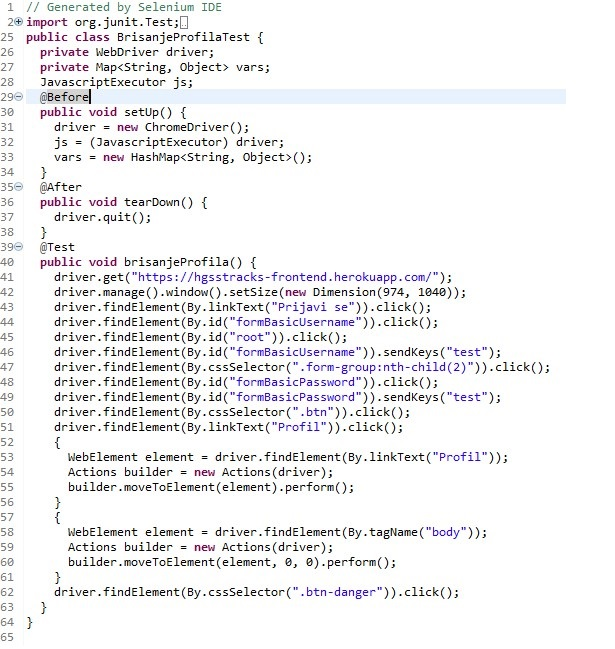
\includegraphics[width=\linewidth]{./slike/BrisanjeProfila.jpg}
					\caption{Prikaz koda ispitivanja \textbf{UC7}}
				\end{figure}
				\eject
			\end{packed_item}
			
			
			
			
			
			
			
			\subsection{Ispitivanje sustava}
			
			 {U sljedećim ispitima funkcionalnosti sustava ispitani su obrasci uporabe \textbf{UC4, UC5,UC24,UC26} i \textbf{UC30}}\\
			 
			 \textbf{Ispitni slučaj 1: Prijava na akciju spašavanja}
			 
			 \textbf{Ulaz:}
			 \begin{itemize}
			 	\item {Prijava u sustav s kredencijama spasioca;}
			 	\item {Pritisak na "Akcije u tijeku" te na jednoj od moguće ponuđenih akcija klik na "Prijavi se na akciju";}
			 	\item {Na "Trenutna Akcija" u \textit{textbox} za ostavljanje komentara ostaviti komentar "SeleniumSelfTest";}
			 	\item {Dojava dispečeru da je osoba pronađena za klikom na gumb "Dojavi".}
			 \end{itemize}
		 	\textbf{Očekivani rezultat:}
		 	\begin{itemize}
		 		\item {Prikazuje se početna stranica;}
		 		\item {Prikazuju se sve aktivne akcije u koje se moguće prijaviti;}
		 		\item {Nakon klika na jednu od akcija očekuje se skočni tekst na samoj stranici koji potvrđuje javljanje na akciju;}
		 		\item {Ostavljanje komentara za dispečera za uvid u akciju na terenu;}
		 		\item {Dojava uspješna da je žrtva nađena.}
		 	\end{itemize}
	 		{\textbf{Rezultat: Svi rezultati su uspješno izvedeni. Aplikacija je prošla test.}}
	 		
			 \begin{figure}[h!]
			 	\centering
			 	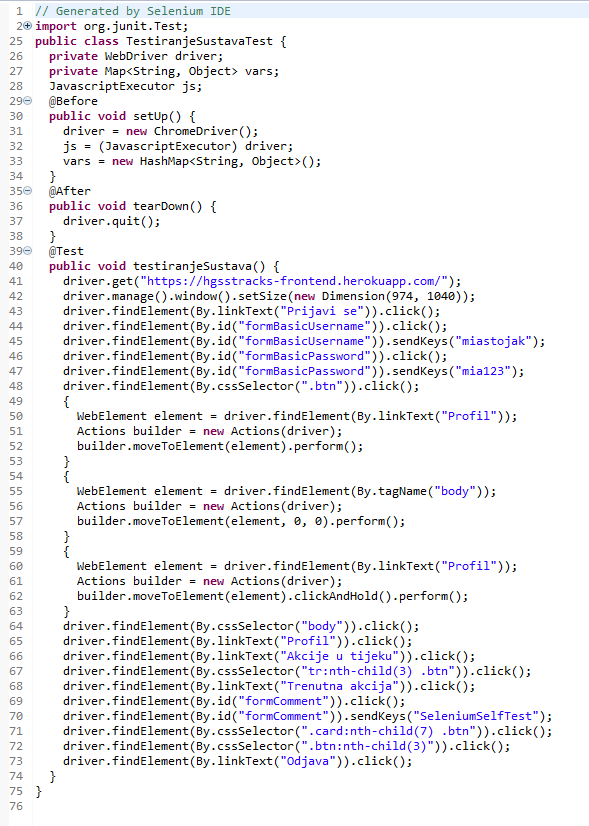
\includegraphics[width=\linewidth]{./slike/IspitivanjeSustava.png}
			 	\caption{Prikaz koda ispitivanja navedenih obrazaca uporabe}
			 \end{figure}
			
			\eject 
			
			\begin{figure}[h!]
				\centering
				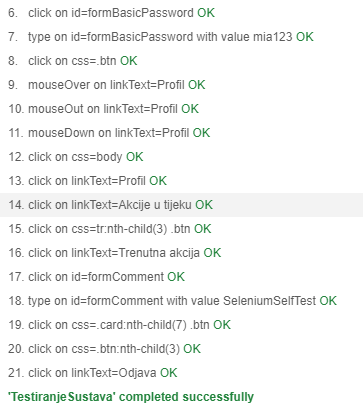
\includegraphics[width=\linewidth]{./slike/TestiranjeRezultat.png}
				\caption{Prikaz Selenium IDE kvalitetu testova}
			\end{figure}
		
			\eject
			
		
		\newpage
		\section{Dijagram razmještaja}
			
			
			 {Dijagram razmještaja na slici ispod prikazuje topologiju komponenti naše aplikacije te programsku potporu iste u radnom okruženju.Na poslužiteljskom računalu se nalazi web poslužitelj aplikacije te baza podataka s informacijama o spasiocima, akcijama, informacijama nestalih osoba, stanicama te ostalih komponenata bitnih za kvalitetan rad aplikacije. Korisnici aplikacije koriste web preglednik kako bi pristupili aplikaciji. Sustav naše aplikacije je baziran na arhitekturi "klijent-poslužitelj", a komunikacija između računala korisnika i poslužitelja odvija se preko HTTP veze.}
			 
			 \begin{figure}[h!]
			 	\centering
			 	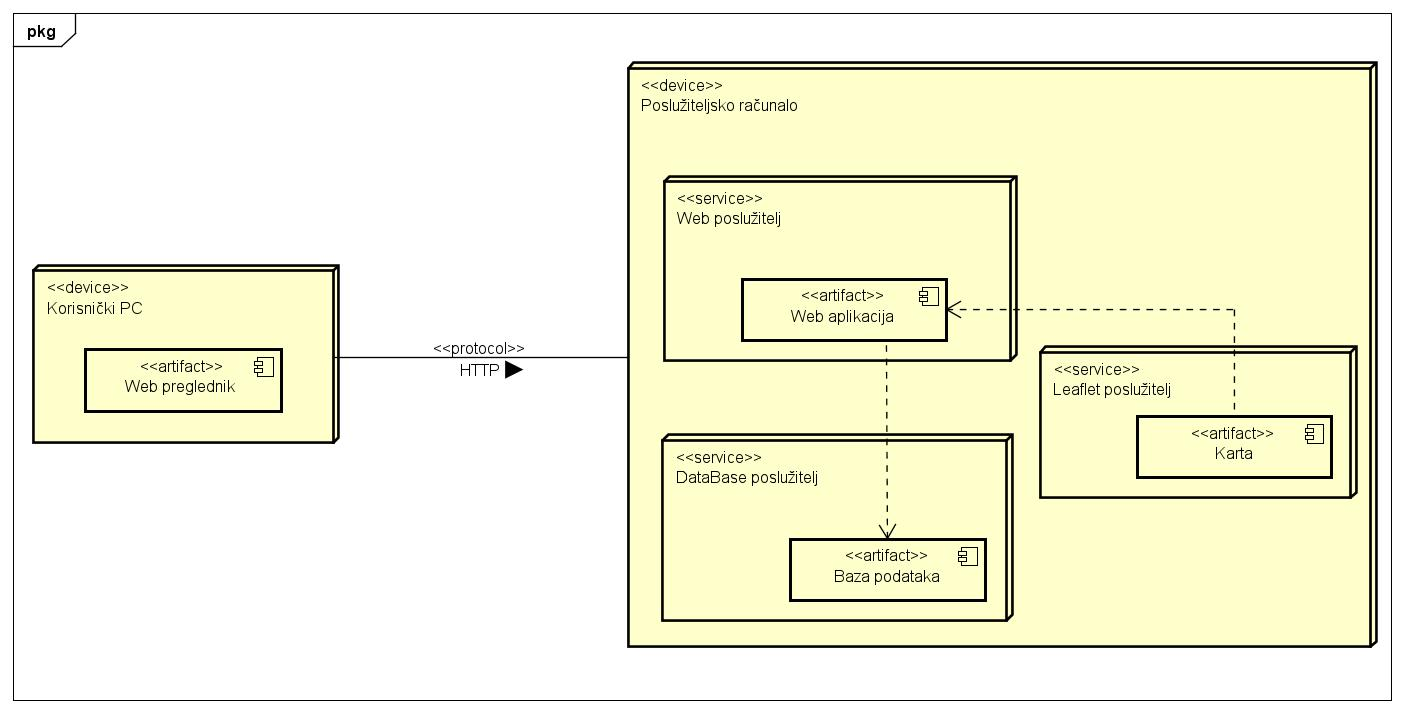
\includegraphics[width=\linewidth]{./slike/Dijagram_razmjestaja.jpg}
			 	\caption{Dijagram razmještaja komponenti}
			 \end{figure}
			
			\eject 
		
		\section{Upute za puštanje u pogon}
		
			\textbf{Instalacija poslužitelja baze podataka}\\
		
			 {Potrebno je preuzeti SQL Shell(Postgress SQL) bazu podataka te pgAdmin radi lakše manipulacije s podatcima tj. bolje preglednosti. Nakon preuzimanja paketa potrebno je provesti standardnu instalaciju s postavljanjem korisnika.}\\
			 
			 \textbf{Konfiguracija poslužitelja baze podataka}\\
			 
			 {Nakon instalacije, uključite pgAdmin server te izvršite prvu konekciju na bazu (s postavljanjem \textit{master} zaporke za pristup).}\\
			 
			 \textbf{Punjenje baze s informacijama}\\
			 
			 {Po prvom paljenju servera baze podataka potrebno je pomoću nekog od uređivača tekstova(notepad,notepad++ itd.) otvoriti datoteku po imenu "Baza.sql" te označiti cijeli tekst i kopirati ga. Kada ste kopirali konfiguraciju baze iz datoteke. Na web poslužitelju pgAdmin potrebno je u padajućem izborniku za "PostgreSQL 13" kliknuti desni klik miša te ići na "New database" te na skočnom prozoru  upisati ime baze, u ovom slučaju "Baza korisnika" te stisnuti "Create". Po izradi baze desni klik na bazu te "Query tool" i na novom prozoru koji će se pojaviti na desnoj strani ekrana zalijepiti tekst iz datoteke "Baza.sql" i pritisnuti gumb "Run".}\\
			 
			 \textbf{Instalacija poslužitelja \textit{backend} koda}\\
			 
			 {Potrebno je preuzeti Eclipse za službene stranice proizvoda. Nakon što se program preuzme potrebno je izvršiti standardnu instalaciju. Također je potrebno u "System variables" postaviti putanju za JAVA HOME.}\\
			 
			 \textbf{Postavljanje putanje za JAVU}\\
			 
			 {Potrebno je otići na "This PC" - desni klik na "This PC" - "Properties" - "Advanced system settings" - "Enviromental variables" - Dvoklik na "Path" - "New". Kada se napravi nova linija potrebno je u nju kopirati tekst "\%JAVA\_HOME\%\textbackslash bin". Nakon toga potrebno je u "Enviromental variables" na donjem dijelu prozoru gdje je "System variables" kliknuti "New" te u "Variable name" upisati "JAVA\_HOME", a u "Variable value" putanju gdje je instaliran JAVA paket na vašem računalu.}\\
			 
			 \textbf{Dodavanje ekstenzija na Eclipse}\\
			 
			 {Nakon instalacije programa Eclipse, te namještanja putanje za JAVA\_HOME potrebno je upaliti program te ići na karticu "Help" - "Eclipse Marketplace" te u find \textit{textboxu} upisati "spring" i instalirati \textit{dashboard} za "Spring Tools 3"(ili trenutnu verziju programa). Nakon instalacije \textit{dashboard}-a potrebno je otići na \textit{\href{https://maven.apache.org/install.html}{https://maven.apache.org/install.html}} te preuzeti paket i instalirati ga na računalo.}\\
			 
			 \textbf{\textit{Importanje backend} dijela aplikacije u Eclipse}\\
			 
			 {Po instalaciji svih potrebnih programa i ekstenzija za \textit{backend} dio aplikacije, otvorite program Eclipse te na kartici "File" - "Import" - "Maven" - "Existing Maven Projects" - "Next" - "Browse" i u skočnom prozoru pronaći datoteku u kojoj je spremljen kod te "Finish". Projektni dio koda je ubačen u Eclipse i moguće je manipulirati s kodom.}\\
			 
			 \textbf{Instalacija \textit{frontend} poslužitelja}\\
			 
			 {Kako bismo mogli vidjeti te preuređivati \textit{frontend} kod potrebno je instalirati program \textit{\textbf{Visual Studio Code}} sa \href{https://code.visualstudio.com/Download}{https://code.visualstudio.com/Download}.}\\
			 
			 \textbf{Instalacija REACT biblioteke u Visual Studio Code program}\\
			 
			 {U svakoj datoteci vezanoj za \textit{frontend} kod potrebno je na početku upisati komande: 
			 import React from 'react';
		 	 import ReactDOM from 'react-dom';
	 	 	 nakon što smo upisali ove dvije komade moguće je koristiti REACT biblioteku u daljnjem kodu.}\\
			
			\textbf{\textit{Importanje frontend} dijela koda u program}\\
			
			{Po instalaciji programa "Visual Studio Code" upalite program te "File" - "Open" te označiti mapu u kojoj se nalaze sve datoteke \textit{frontend} dijela projekta. Po uspješnom otvaranju datoteka moguće je manipulirati kodom.}\\
			
			\textbf{\textit{Deploy backend} dijela projekta na Heroku}\\
			
			{U datoteku "pom.xml" potrebno je dodati maven plugin za \textbf{Heroku} čiji je dependency moguće naći na \href{https://elements.heroku.com/buildpacks/heroku/heroku-maven-plugin}{ovom linku}. Nakon dodavanja "dependency-ja" upalite git bash te se pozicionirati u mapu u kojoj se nalazi projekt. U "Git-bash" je potrebno upisati naredbu heroku git:remote -a hgsstracks-backend. Informacije o bazi podataka za aplikaciju moguće je naredbom heroku pg:info. Iz informacija koje smo dobili o bazi podataka potrebno je iščitati <Add-on>. Kada smo iščitali <Add-on> napunićemo bazu podataka informacijama koje imamo u mapi "Izvršni kod" upišemo naredbu heroku pg:psql <Add-on> --app <name\_of\_app> < my\_sql\_file.sql;, u našem slučaju ta naredba glasi heroku pg:psql postgresql-curly-47290 --app hgsstracks-backend < Baza.sql. U datoteci application.properties je potrebno postaviti informacije o bazi tj. ime baze podataka te zaporku za istu koju smo postavili u prethodnim koracima. Nakon punjenja baze pozovemo naredbu mvn clean heroku:deploy te je s time \textit{backend} dio projekta pušten u pogon.}\\
			
			\textbf{\textit{Deploy frontend} dijela projekta na Heroku}\\
			
			{U vršnu mapu projekta potrebno je dodati datoteku "package.json" s naredbama "heroku-prebuild": "cd \"Izvorni kod"/frontend/hgsstracks\" i start": "start": "cd \"Izvorni kod"/frontend/hgsstracks/\" \&\& npm start" te naposljetku "build": "cd \"Izvorni kod"/frontend/hgsstracks\" \&\& react-scripts build". Nakon izvedbe naredbi u "package.json" unutar \textit{frontend} mape potrebno je promijeniti skripte u "start": "npm install -g serve \&\& serve -s build". Upalimo "Git-bash" te se pozicioniramo u njemu u mapu u kojoj se nalazi naš \textit{frontend} dio projekta te upišemo naredbu heroku git:remote -a hgsstracks-frontend. Pozovemo naredbu git push heroku <branch>:main, u našem slučaju ta naredba je git push heroku develop:main. \textit{Frontend} dio projekta je pušten u pogon.}\\
			
			
			
			
			\eject 
	\chapter{Zaključak i budući rad}
		
		
	 		{Zadatak naše grupe bio je napraviti web aplikaciju za ubrzano 	javljanje informacija o nestalim osobama te javljanje spasilaca na akcije spašavanja istih. Nakon dva ciklusa nastave i praznika, ostvarili smo cilj koji nam je zadan. Rad na aplikaciji razdijeljen je bio na tri faze.\\
	 			Prva faza sastojala se od okupljanja članova tima koji će razvijati aplikaciju, dodjelu projektnog zadatka te rada na dokumentiranju zahtjeva i osmišljaju najboljeg tijeka rada.\\
	 			Druga faza rada na aplikaciji bila je rezervirana za izradu osnovnih funkcija to jest za generalnu funkcionalnost aplikacije (prijava korisnika u sustav). Za vrijeme izrade generalne funkcionalnosti došlo je do nekoliko problema koji su rezultirali mijenjanjem do tada korištene tehnologije na novu,uvod JPA u projekt, kako bismo mogli lakše manipulirati s podatcima u bazi podataka. Prije prve predaje osnovne inačice aplikacije također su izrađeni obrasci i dijagrami(obrasci uporabe,sekvencijski dijagrami, model baze podataka i dijagrami razreda). Izrada ovih idejnih dijelova dokumentacije kasnije je služila \textit{frontend} i \textit{backend} timovima kao osnova za razvoj daljnjih funkcija aplikacije.\\
	 			Treća faza realizacije aplikacije bila je najintenzivniji dio rada na aplikaciji. Intenzitet je pristizao od neiskustva članova timova s novim tehnologijama korištenima u projektu. Timovi su bili zaduženi za izradu ostalih dijelova zahtjeva za projekt, točnije dijelova aplikacije za razne vrste korisnika kao i samog admina aplikacije. Uz rad na funkcionalnostima također su napravljeni i ostali UML dijagrami i ostatak dokumentacije koja će služiti budućim korisnicima kao naputak za korištenje i snalaženje u slučaju preinake sustava. Izvrsno izrađen kostur aplikacije služio je \textit{backend} i \textit{frontend} timovima kao ubrzanje rada zato što je lakše bilo izbjegavati eventualne pogreške koje bi koštale sati rada na aplikaciji bez uroda.\\ 
	 			Komunikacija između članova većinski je rađeno preko WhatsApp aplikacije te timskog rada na Discord-u. Moguć daljnji napredak aplikacije značio bi izrada mobilne aplikacije koja bi značila ostvarenje i više nego što je bio cilj.\\
	 			Sudjelovanje u izradi web aplikacije bilo je vrijedno iskustvo svim članovima tima zbog intenziteta rada, te učenja novih tehnologija. Uz rad i nove tehnologije tim je također naučio i važnost dobre koordinacije članova time kao i vremenske organiziranosti, koja je značila izradu projekta u predviđenom vremenu. Naš tim je iznimno zadovoljan dostignutim ciljem usprkos moguće dorade i usavršavanja samog projekta bez obzira na minimalno ili nikakvo iskustvo u ovakvim projektima i tehnologija.
	 	 } 
		
		\eject 
	\chapter*{Popis literature}
		\addcontentsline{toc}{chapter}{Popis literature}
	 	
		
		
		\begin{enumerate}
			
			
			\item  Programsko inženjerstvo, FER ZEMRIS,\\ \url{http://www.fer.hr/predmet/proinz}
			
			\item  Hrvatski crveni križ,\\
			\url{http://www2.hck.hr/hr}
			
			\item  The Unified Modeling Language,\\ \url{https://www.uml-diagrams.org/}
			
			\item  Astah Community, \\
			\url{http://astah.net/editions/uml-new}
			
			\item  PostgreSQL, \\
			\url{https://jdbc.postgresql.org/}
			
			
		\end{enumerate}
		
		 
	
	
	\begingroup
	\renewcommand*\listfigurename{Indeks slika i dijagrama}
	%\renewcommand*\listtablename{Indeks tablica}
	%\let\clearpage\relax
	\listoffigures
	%\vspace{10mm}
	%\listoftables
	\endgroup
	\addcontentsline{toc}{chapter}{Indeks slika i dijagrama}


	
	\eject 
		
	\chapter*{Dodatak: Prikaz aktivnosti grupe}
		\addcontentsline{toc}{chapter}{Dodatak: Prikaz aktivnosti grupe}
		
		\section*{Dnevnik sastajanja\\}
		
		\begin{packed_enum}
			
		
			\item  sastanak
			
			\item[] \begin{packed_item}
				\item Datum:  8.listopada 2020.
				\item Prisustvovali: B.Boras, L.Gusar, K.Kovać, Z.F.Kovačić, S.Mlakić, M.Škrabić, M.Stojak
				\item Teme sastanka:
				\begin{packed_item}
					\item  Pitanja o temi
					\item  Sastanak s asistentom i demonstratorom
					\item  Raščišćavanje osnovnih dilema funkcionalnosti
					\item  Analiza zadatka\\
				\end{packed_item}
			\end{packed_item}

			\item  sastanak
		
			\item[] \begin{packed_item}
				\item Datum:  7.listopada 2020.
				\item Prisustvovali: H.Nuić, B.Boras, L.Gusar, K.Kovać, Z.F.Kovačić, S.Mlakić, M.Škrabić, M.Stojak
				\item Teme sastanka:
				\begin{packed_item}
					\item  Uvodni sastanak\\
				\end{packed_item}
			\end{packed_item}
		
			\item  sastanak
			
			\item[] \begin{packed_item}
				\item Datum: 13. listopada 2020.
				\item Prisustvovali: S.Mlakić, L.Gusar
				\item Teme sastanka:
				\begin{packed_item}
					\item  Relacije baze podataka
					\item  Entiteti baze podataka\\
				\end{packed_item}
			\end{packed_item}
			\newpage
			\item  sastanak
			\item[] \begin{packed_item}
				\item Datum: 19. listopada 2020.
				\item Prisustvovali: B.Boras, L.Gusar, K.Kovać, Z.F.Kovačić, S.Mlakić, M.Škrabić, M.Stojak
				\item Teme sastanka:
				\begin{packed_item}
					\item  Početak rada frontenda i backenda
					\item  Raspodjela poslova(funkcionalni zahtjevi + obrasci uporabe + dijagrami)
					\item  Diskutiranje o izgledu stranice i funkcijama\\
				\end{packed_item}
			\end{packed_item}
		
			\item  sastanak
			
			\item[] \begin{packed_item}
				\item Datum:  21.listopada 2020.
				\item Prisustvovali: H.Nuić, B.Boras, L.Gusar, K.Kovać, Z.F.Kovačić, S.Mlakić, M.Škrabić, M.Stojak
				\item Teme sastanka:
				\begin{packed_item}
					\item  Razjašnjavanje problema\\
				\end{packed_item}
			\end{packed_item}
		
			\item  sastanak
			\item[] \begin{packed_item}
				\item Datum: 21. listopada 2020.
				\item Prisustvovali: B.Boras, L.Gusar, Z.F.Kovačić, S.Mlakić, M.Škrabić, M.Stojak
				\item Teme sastanka:
				\begin{packed_item}
					\item  Određivanje funkcionalnih zahtjeva\\
				\end{packed_item}
			\end{packed_item}
		
			\item  sastanak
			\item[] \begin{packed_item}
				\item Datum: 28. listopada 2020.
				\item Prisustvovali:  B.Boras, L.Gusar, Z.F.Kovačić, M.Škrabić, M.Stojak
				\item Teme sastanka:
				\begin{packed_item}
					\item  Povezivanje backenda i frontenda\\
				\end{packed_item}
			\end{packed_item}
		\newpage
			\item  sastanak
			
			\item[] \begin{packed_item}
				\item Datum:  1. studenoga 2020.
				\item Prisustvovali: B.Boras, L.Gusar, K.Kovać, Z.F.Kovačić, S.Mlakić, M.Škrabić, M.Stojak
				\item Teme sastanka:
				\begin{packed_item}
					\item  Sistematizacija stavki koje se trebaju napraviti za 1. reviziju
					\item  Rješavanje problema\\
				\end{packed_item}
			\end{packed_item}
		
			\item sastanak
			
			\item[] \begin{packed_item}
				\item Datum:  6. studenoga 2020.
				\item Prisustvovali: K.Kovać, Z.F.Kovačić, M.Škrabić
				\item Teme sastanka:
				\begin{packed_item}
					\item  Razjašnjavanje problema o dokumentaciji i implementaciji\\
				\end{packed_item}
			\end{packed_item}
			
			\item  sastanak
			
			\item[] \begin{packed_item}
				\item Datum:  9. studenoga 2020.
				\item Prisustvovali: H.Nuić, B.Boras, L.Gusar, K.Kovać, Z.F.Kovačić, S.Mlakić, M.Škrabić, M.Stojak
				\item Teme sastanka: 
				\begin{packed_item}
					\item  Razjašnjavanje problema o dokumentaciji i implementaciji\\ 
				\end{packed_item}
			\end{packed_item}
			
			\item sastanak
			
			\item[] \begin{packed_item}
				\item Datum:  3. prosinca 2020.
				\item Prisustvovali: H.Nuić, B.Boras, L.Gusar, K.Kovać, Z.F.Kovačić, S.Mlakić, M.Škrabić, M.Stojak
				\item Teme sastanka:
				\begin{packed_item}
					\item  Ispitivanje\\
				\end{packed_item}
			\end{packed_item}
		
			\item sastanak
			
			\item[] \begin{packed_item}
				\item Datum:  4. prosinca 2020.
				\item Prisustvovali: B.Boras, L.Gusar, K.Kovać, Z.F.Kovačić, S.Mlakić, M.Škrabić, M.Stojak
				\item Teme sastanka:
				\begin{packed_item}
					\item  Dogovor što dalje
					\item  Raspodjela osoba u timu\\
				\end{packed_item}
			\end{packed_item}
			
			\item sastanak
			
			\item[] \begin{packed_item}
				\item Datum:  12. prosinca 2020.
				\item Prisustvovali: B.Boras, L.Gusar, K.Kovać, Z.F.Kovačić, S.Mlakić, M.Škrabić, M.Stojak
				\item Teme sastanka:
				\begin{packed_item}
					\item  Dogovor zadataka
					\item  Prolazak kroz funkcijske zahtjeve i određivanje prioriteta\\
				\end{packed_item}
			\end{packed_item}
			
			\item sastanak
			
			\item[] \begin{packed_item}
				\item Datum:  18. prosinca 2020.
				\item Prisustvovali: B.Boras, L.Gusar, K.Kovać, Z.F.Kovačić, S.Mlakić, M.Škrabić, M.Stojak
				\item Teme sastanka:
				\begin{packed_item}
					\item  Sistematizacija što je završeno
					\item  Prolazak kroz ostale funkcijske zahtjeve\\
				\end{packed_item}
			\end{packed_item}
		
			\item[] \begin{packed_item}
				\item Datum:  21. prosinca 2020.
				\item Prisustvovali: B.Boras, L.Gusar, K.Kovać, Z.F.Kovačić,  M.Škrabić, M.Stojak
				\item Teme sastanka:
				\begin{packed_item}
					\item  Dogovor za simulaciju alfa verzije projekta\\
				\end{packed_item}
			\end{packed_item}
		
			\item[] \begin{packed_item}
				\item Datum:  21. prosinca 2020.
				\item Prisustvovali: L.Gusar, Z.F.Kovačić, S.Mlakić, M.Škrabić, M.Stojak
				\item Teme sastanka:
				\begin{packed_item}
					\item  Simulacija demonstracije alfa verzije projekta\\
				\end{packed_item}
			\end{packed_item}
			
		\end{packed_enum}
			
		
		\eject
		\section*{Tablica aktivnosti}
					
						
			
			\begin{longtabu} to \textwidth {|X[7, l]|X[1, c]|X[1, c]|X[1, c]|X[1, c]|X[1, c]|X[1, c]|X[1, c]|}
								
				\cline{2-8} \multicolumn{1}{c|}{\textbf{}} &     \multicolumn{1}{c|}{\rotatebox{90}{\textbf{Mia Stojak}}} & \multicolumn{1}{c|}{\rotatebox{90}{\textbf{Bartol Boras}}} &	\multicolumn{1}{c|}{\rotatebox{90}{\textbf{Lovre Gusar}}} &	\multicolumn{1}{c|}{\rotatebox{90}{\textbf{Karlo Kovać }}} &
				\multicolumn{1}{c|}{\rotatebox{90}{\textbf{Zrin Franko Kovačić   }}} &
				\multicolumn{1}{c|}{\rotatebox{90}{\textbf{Stjepan Mlakić }}} &	\multicolumn{1}{c|}{\rotatebox{90}{\textbf{Matej Škrabić }}} \\ \hline 
				\endfirsthead
				
			
				\cline{2-8} \multicolumn{1}{c|}{\textbf{}} &     \multicolumn{1}{c|}{\rotatebox{90}{\textbf{Mia Stojak}}} & \multicolumn{1}{c|}{\rotatebox{90}{\textbf{Bartol Boras}}} &	\multicolumn{1}{c|}{\rotatebox{90}{\textbf{Lovre Gusar}}} &	\multicolumn{1}{c|}{\rotatebox{90}{\textbf{Karlo Kovać }}} &
				\multicolumn{1}{c|}{\rotatebox{90}{\textbf{Zrin Franko Kovačić   }}} &
				\multicolumn{1}{c|}{\rotatebox{90}{\textbf{Stjepan Mlakić }}} &	\multicolumn{1}{c|}{\rotatebox{90}{\textbf{Matej Škrabić }}} \\ \hline 
				\endhead
				
				
				\endfoot
							
				 
				\endlastfoot
				
				Upravljanje projektom 		&20  &  &  &  &  &  & \\ \hline
				Opis projektnog zadatka 	&3  &  &  &  &2  &  & \\ \hline
				
				Funkcionalni zahtjevi       &00:10  &00:10  &00:10  &00:10  &00:10  &00:10  &00:10  \\ \hline
				Opis pojedinih obrazaca 	&1  &2  &1  &1  &1  &1  &1  \\ \hline
				Dijagram obrazaca 			&1  &  &  &  &  &3  &  \\ \hline
				Sekvencijski dijagrami 		&1  &  &  &  &  &  &3  \\ \hline
				Opis ostalih zahtjeva 		&  &00:20  &  &  &  &  &  \\ \hline

				Opis arhitekture sustava	 &  &  &3  &  &  &  &  \\ \hline
				Dijagram baze podataka	 &00:30  &  &1  &  &  &  &  \\ \hline
				Baza podataka				&  &  &15  &  &  &15  &   \\ \hline
				Dijagram razreda 			&  &  &  &  &2  &  &   \\ \hline
				Dijagram stanja				&  &  &  &  &1  &  &  \\ \hline
				Dijagram aktivnosti 		&  &  &  &  &2  &  &  \\ \hline
				Dijagram komponenti			&  &  &  &  &2  &  &  \\ \hline
				Korištene tehnologije i alati 		&  &  &1  &  &1  &  &  \\ \hline
				Ispitivanje programskog rješenja 	&2  &  &  &  &2  &  &  \\ \hline
				Dijagram razmještaja			&  &  &  &  &2  &  &  \\ \hline
				Upute za puštanje u pogon 		&1  &  &  &  &3  &  &  \\ \hline 
				Dnevnik sastajanja 			&2  &  &  &  &  &  &  \\ \hline
				Pravopis i uređivanje dokumentacije 		&4  &  &  &  &  &  &  \\  \hline
				Popis literature 			&1  &  &  &  &  &  &  \\  \hline
				Backend			&  &  &  &40  &40  &  &  \\  \hline
				Frontend		&  &40  &  &  &  &  &50\\  \hline
				
				
			\end{longtabu}
					
					
		\eject
		\section*{Dijagrami pregleda promjena}
		
		
		\begin{packed_item}
			\item \textbf{\textit{Grana master}}\\
			
			\begin{figure}[h!]
				\centering
				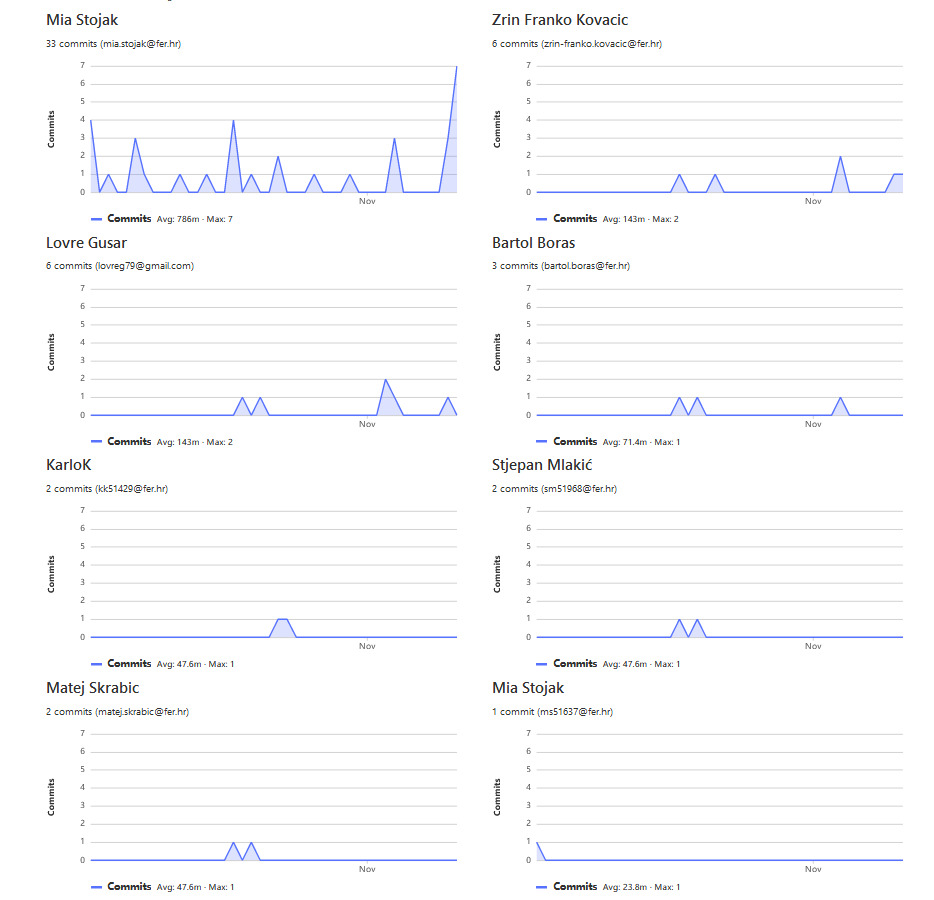
\includegraphics[width=\linewidth]{./slike/master.jpeg}
				\caption{master}
			\end{figure}
			\eject
		\end{packed_item}
	
		\begin{packed_item}
			\item \textbf{\textit{Grana devdoc}}\\
			
			\begin{figure}[h!]
				\centering
				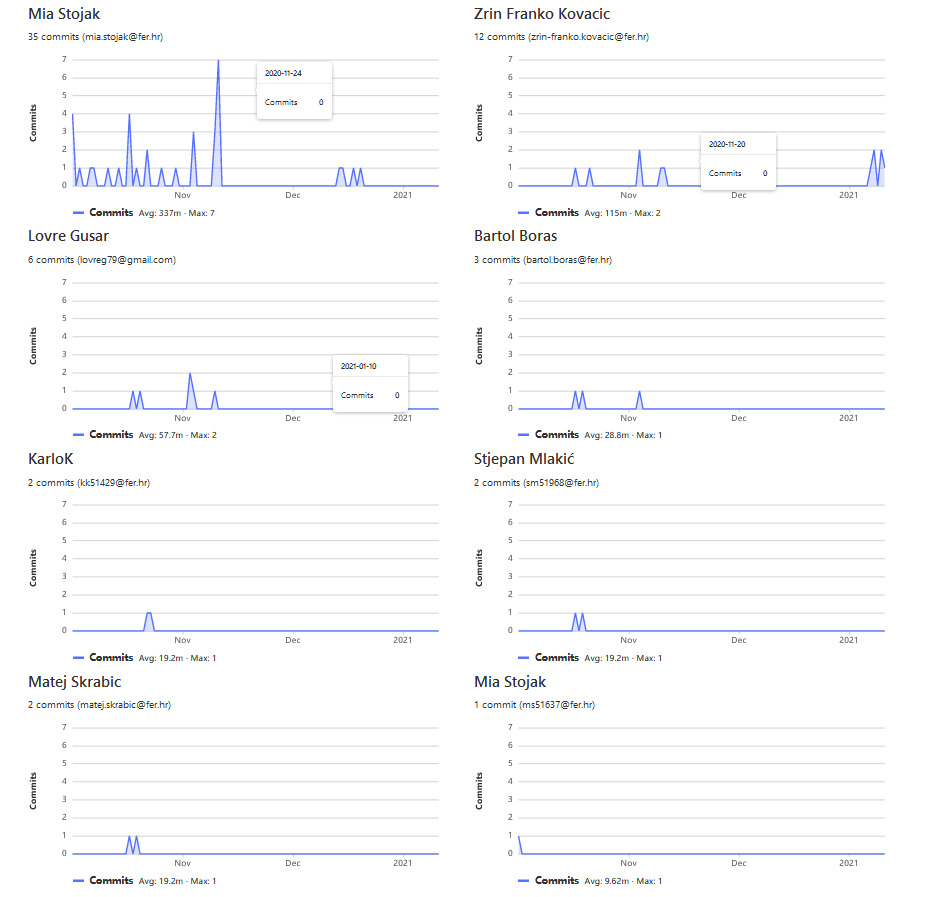
\includegraphics[width=\linewidth]{./slike/devdoc.jpeg}
				\caption{devdoc}
			\end{figure}
			\eject
		\end{packed_item}
	
	\begin{packed_item}
		\item \textbf{\textit{Grana develop}}\\
		
		\begin{figure}[h!]
			\centering
			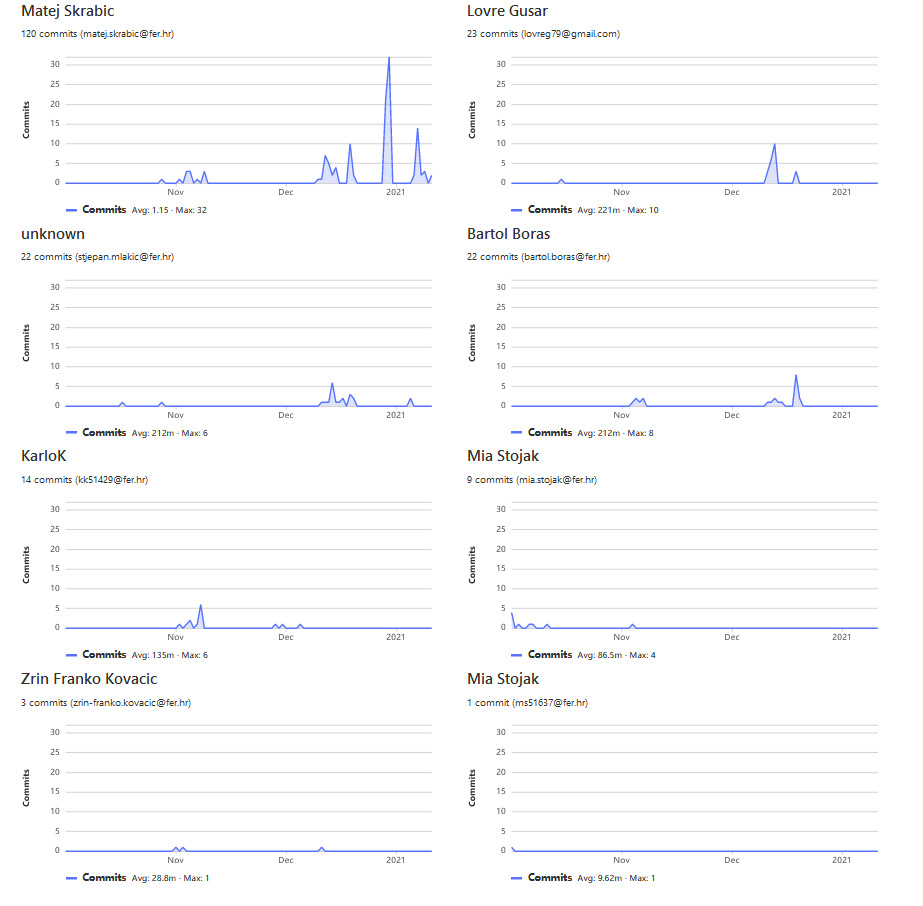
\includegraphics[width=\linewidth]{./slike/develop.jpeg}
			\caption{develop}
		\end{figure}
		\eject
	\end{packed_item}

		\begin{packed_item}
			\item \textbf{\textit{Grana baza}}\\
			
			\begin{figure}[h!]
				\centering
				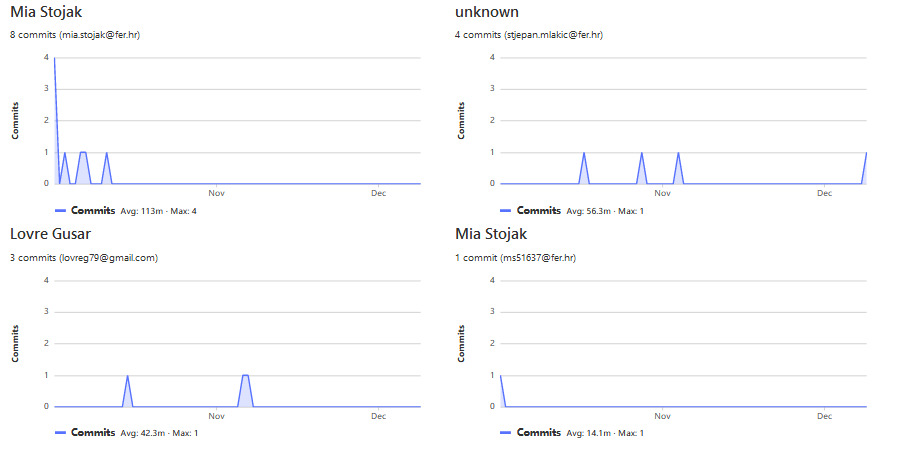
\includegraphics[width=\linewidth]{./slike/baze.jpeg}
				\caption{baza}
			\end{figure}
			\eject
		\end{packed_item}
		
	


\end{document} %naredbe i tekst nakon ove naredbe ne ulaze u izgrađen dokument 


